\documentclass[,man,floatsintext]{apa6}
\usepackage{lmodern}
\usepackage{amssymb,amsmath}
\usepackage{ifxetex,ifluatex}
\usepackage{fixltx2e} % provides \textsubscript
\ifnum 0\ifxetex 1\fi\ifluatex 1\fi=0 % if pdftex
  \usepackage[T1]{fontenc}
  \usepackage[utf8]{inputenc}
\else % if luatex or xelatex
  \ifxetex
    \usepackage{mathspec}
  \else
    \usepackage{fontspec}
  \fi
  \defaultfontfeatures{Ligatures=TeX,Scale=MatchLowercase}
\fi
% use upquote if available, for straight quotes in verbatim environments
\IfFileExists{upquote.sty}{\usepackage{upquote}}{}
% use microtype if available
\IfFileExists{microtype.sty}{%
\usepackage{microtype}
\UseMicrotypeSet[protrusion]{basicmath} % disable protrusion for tt fonts
}{}
\usepackage{hyperref}
\hypersetup{unicode=true,
            pdftitle={Children flexibly seek visual information during signed and spoken language comprehension},
            pdfauthor={Kyle MacDonald, Virginia A. Marchman, Anne Fernald, \& Michael C. Frank},
            pdfkeywords={eye movements; grounded language comprehension; information-seeking; speech in background noise; American Sign Language},
            pdfborder={0 0 0},
            breaklinks=true}
\urlstyle{same}  % don't use monospace font for urls
\usepackage{graphicx,grffile}
\makeatletter
\def\maxwidth{\ifdim\Gin@nat@width>\linewidth\linewidth\else\Gin@nat@width\fi}
\def\maxheight{\ifdim\Gin@nat@height>\textheight\textheight\else\Gin@nat@height\fi}
\makeatother
% Scale images if necessary, so that they will not overflow the page
% margins by default, and it is still possible to overwrite the defaults
% using explicit options in \includegraphics[width, height, ...]{}
\setkeys{Gin}{width=\maxwidth,height=\maxheight,keepaspectratio}
\IfFileExists{parskip.sty}{%
\usepackage{parskip}
}{% else
\setlength{\parindent}{0pt}
\setlength{\parskip}{6pt plus 2pt minus 1pt}
}
\setlength{\emergencystretch}{3em}  % prevent overfull lines
\providecommand{\tightlist}{%
  \setlength{\itemsep}{0pt}\setlength{\parskip}{0pt}}
\setcounter{secnumdepth}{0}
% Redefines (sub)paragraphs to behave more like sections
\ifx\paragraph\undefined\else
\let\oldparagraph\paragraph
\renewcommand{\paragraph}[1]{\oldparagraph{#1}\mbox{}}
\fi
\ifx\subparagraph\undefined\else
\let\oldsubparagraph\subparagraph
\renewcommand{\subparagraph}[1]{\oldsubparagraph{#1}\mbox{}}
\fi

%%% Use protect on footnotes to avoid problems with footnotes in titles
\let\rmarkdownfootnote\footnote%
\def\footnote{\protect\rmarkdownfootnote}


  \title{Children flexibly seek visual information during signed and spoken language comprehension}
    \author{Kyle MacDonald\textsuperscript{1, 2}, Virginia A. Marchman\textsuperscript{1}, Anne Fernald\textsuperscript{1}, \& Michael C. Frank\textsuperscript{1}}
    \date{}
  
\shorttitle{Revision of XGE-2018-1527 as invited by the action editor, Cathie Tamis-LeMonda.}
\affiliation{
\vspace{0.5cm}
\textsuperscript{1} Stanford University\\\textsuperscript{2} University of California, Los Angeles}
\keywords{eye movements; grounded language comprehension; information-seeking; speech in background noise; American Sign Language\newline\indent Word count: 9323}
\usepackage{csquotes}
\usepackage{upgreek}
\captionsetup{font=singlespacing,justification=justified}

\usepackage{longtable}
\usepackage{lscape}
\usepackage{multirow}
\usepackage{tabularx}
\usepackage[flushleft]{threeparttable}
\usepackage{threeparttablex}

\newenvironment{lltable}{\begin{landscape}\begin{center}\begin{ThreePartTable}}{\end{ThreePartTable}\end{center}\end{landscape}}

\makeatletter
\newcommand\LastLTentrywidth{1em}
\newlength\longtablewidth
\setlength{\longtablewidth}{1in}
\newcommand{\getlongtablewidth}{\begingroup \ifcsname LT@\roman{LT@tables}\endcsname \global\longtablewidth=0pt \renewcommand{\LT@entry}[2]{\global\advance\longtablewidth by ##2\relax\gdef\LastLTentrywidth{##2}}\@nameuse{LT@\roman{LT@tables}} \fi \endgroup}

\authornote{

Correspondence concerning this article should be addressed to Kyle MacDonald, 2225 Rolfe Hall, Los Angeles, CA 90095. E-mail: \href{mailto:kemacdonald@ucla.edu}{\nolinkurl{kemacdonald@ucla.edu}}}

\abstract{
During grounded language comprehension, listeners must link the incoming linguistic signal to the visual world despite noise in the input. Information gathered through visual fixations can facilitate understanding. But do listeners flexibly seek supportive visual information? Here, we propose that even young children can adapt their gaze and actively gather information that supports their language understanding. We present two studies of eye movements during real-time language processing where the value of fixating on a social partner varies across different contexts. First, compared to children learning spoken English (n=80), young American Sign Language (ASL) learners (n=30) delayed gaze shifts away from a language source and produced a higher proportion of language-consistent eye movements. This result suggests that ASL learners adapt to dividing attention between language and referents, which both compete for processing via the same channel: vision. Second, English-speaking preschoolers (n=39) and adults (n=31) delayed the timing of gaze shifts away from a speaker's face while processing language in a noisy auditory environment. This delay resulted in a higher proportion of language-consistent gaze shifts. These results suggest that young listeners can adapt their gaze to seek supportive visual information from social partners during real-time language comprehension.


}

\begin{document}
\maketitle

\hypertarget{introduction}{%
\section{Introduction}\label{introduction}}

Extracting meaning from language represents a formidable challenge for young learners. Consider that even in the simple case of understanding grounded, familiar language (e.g., \enquote{look at the ball}), listeners must quickly integrate linguistic and non-linguistic information from two continuous streams of input. Moreover, words occur within dynamic interactions where there is often insufficient information to figure out what is being said, and yet listeners must decide how best to respond. Even young children are capable of linking language to the world quite efficiently, shifting visual attention to a named object in a scene within hundreds of milliseconds upon hearing its name in controlled laboratory conditions (Fernald, Perfors, \& Marchman, 2006). But how do children comprehend language when processing demands are higher and the input is noisy?

In interactive theories of language comprehension, listeners integrate noisy input from multiple sources of information to constrain the set of possible interpretations of an utterance (MacDonald \& Seidenberg, 2006; McClelland \& Elman, 1986). Under this interactive account, listeners comprehend words by partially activating several candidates that are consistent with incoming perceptual information. As more information arrives, words that do not match the perceptual signal are no longer considered, and words that do match become more strongly activated until a single interpretation is reached (see McClelland, Mirman, and Holt, 2006, for a review). Critically, multiple sources of information -- the linguistic signal, visual world, and conceptual knowledge -- mutually influence one another to constrain the listener's interpretation of an utterance (e.g., the \enquote{McGurk effect} {[}MacDonald \& McGurk, 1978{]} and parsing syntactically ambiguous utterances {[}Tanenhaus, Spivey-Knowlton, Eberhard, \& Sedivy, 1995{]}).

Thus, visual information can facilitate language comprehension. But the incoming visual and linguistic signals are transient, and rather than randomly fixate a scene, listeners might strategically deploy fixations to informative locations. Consider a speaker who asks you to \enquote{Pass the salt} in a noisy restaurant where it is difficult to perceive what she is saying. Recent theoretical and empirical work suggests that children and adults can overcome a \enquote{noisy signal} by integrating what they perceive with their prior beliefs about what the speaker was likely to have said (Fourtassi \& Frank, 2017; Gibson, Bergen, \& Piantadosi, 2013; Yurovsky, Case, \& Frank, 2017). In the current work, we pursue a variant of this idea and ask whether listeners strategically gather visual information that could be integrated with the linguistic signal to comprehension.

Another case where the strategic use of visual fixations becomes necessary is the comprehension of visual-manual languages such as American Sign Language (ASL). In ASL, looks to the language source are highly informative because signers must process the linguistic information via the visual channel. Further, the decision to look away from a signer to the rest of the visual world risks reducing access to subsequent linguistic information, thus complicating the decision to gather other, potentially-relevant visual information. ASL also represents a case where there is direct competition between allocating visual attention to non-linguistic cues -- e.g., gesture, eye gaze, and facial expressions -- that have been proposed to support spoken language comprehension. This competition for visual attention raises an interesting question about whether learning ASL would result in an adaptation of how children choose to distribute gaze across multiple, potententially language-relevant locations when processing language in real-time.

Taken together, the ASL and noisy restaurant examples highlight how eye movements could reflect an active process of gathering language-relevant information. In the current work, we pursue this idea and propose that listeners are sensitive to the value of different fixation behaviors for the goal of grounded language understanding. We hypothesize that even young children can flexibly adapt the dynamics of their gaze to seek higher value visual information that supports comprehension. This proposal extends prior work on children's eye movements during language understanding, which has tended to focus on gaze shits as the output of the comprehension process. Moreover, by considering listeners' goals and knowledge, the current work moves beyond accounts that explain eye movements in terms of properties of the external scene (e.g., salience of objects) without considering processes internal to the listener (e.g., goals).

Several research programs inspired our hypothesis, including work on language-driven shifts in visual attention (Allopenna, Magnuson, \& Tanenhaus, 1998; Tanenhaus, Spivey-Knowlton, Eberhard, \& Sedivy, 1995), goal-based accounts of eye movements in everyday tasks (Hayhoe \& Ballard, 2005; Henderson, 2017), and language perception as a process of multisensory cue integration (Vigliocco, Perniss, \& Vinson, 2014). In the following three sections, we briefly review each literature to highlight the contribution of characterizing eye movements as seeking language-relevant information during grounded signed and spoken language understanding.

\hypertarget{vision-language-interactions-during-language-comprehension}{%
\subsection{Vision-language interactions during language comprehension}\label{vision-language-interactions-during-language-comprehension}}

The study of eye movements during spoken language comprehension has provided insight into the interaction between concepts, language, and visual attention. The majority of this work has used the Visual World Paradigm (VWP) where listeners' eye movements are recorded at the millisecond timescale while processing language and looking at a set of objects (see Salverda, Brown, \& Tanenhaus, 2011, for a review). Crucially, these analyses rely on the fact that listeners will initiate gaze shifts to named referents with only partial information, in contrast to waiting until the end of a cognitive process (Gold \& Shadlen, 2000). Thus, the time course of eye movements can provide a window onto how and when people integrate information to reach an interpretation of the incoming linguistic signal.

A classic finding using the VWP shows that listeners will rapidly shift visual attention upon hearing the name of an object (\enquote{Pick up a beaker.}) in the visual scene with a high proportion of shifts occurring soon after the target word begins (Allopenna et al., 1998). Moreover, adults will look at a phonological onset-competitor (\enquote{beetle}) early upon hearing the word \enquote{beaker,} suggesting that they activate multiple interpretations and resolve ambiguity as the stimulus unfolds. Information from the visual world can also constrain interpretation by activating listeners' conceptual representations before the arrival of the linguistic signal (Dahan \& Tanenhaus, 2005; Yee \& Sedivy, 2006). These results confirm predictions made by interactive models of speech perception where information from multiple sources is integrated rapidly to constrain language understanding (MacDonald \& Seidenberg, 2006; McClelland, Mirman, \& Holt, 2006).

In addition to work in adult psycholinguistics, the VWP has been useful for studying developmental change in language comprehension skill in children. Researchers have adapted the task to measure the timing and accuracy of children's gaze shifts as they look at two familiar objects and listen to simple sentences naming one of the objects (Fernald, Zangl, Portillo, \& Marchman, 2008; Venker, Eernisse, Saffran, \& Weismer, 2013). Such research finds that children, like adults, shift gaze to named objects soon after the acoustic information is sufficient to enable referent identification. Further, individual differences in the speed and accuracy of eye movements predict vocabulary growth and later language and cognitive outcomes (Fernald et al., 2006; Marchman \& Fernald, 2008; Rigler et al., 2015).

Taken together, the research on children's distribution of gaze during language comprehension shows that the effect of spoken language on visual attention is quite rapid and that eye movements reflect the real-time activation of conceptual information related to the linguistic signal. This work has leveraged eye movements as the output measure of children's language comprehension, focusing less on whether eye movements might also reflect strategic information-gathering process driven by the goal to understand one's communicative partner. Moreover, the existing work raises an interesting question about the extent to which language-related eye movements are driven by external (e.g., salience) vs.~internal (e.g., goals) processes, and whether this relationship might change as a function of children's developing linguistic knowledge.

In the current studies, we use the VWP to addresss this open question and ask whether children strategically adapt their eye movements to seek information in response to the processing demands of their environment. By characterizing eye movements as an index of seeking language-relevant information, we go beyond prior work on children's gaze during language comprehension, which has tended to analyze eye movements as the output of language comprehension. This shift in the construal of eye movements was inspired by work on goal-based accounts of vision that start from the idea that gaze shifts reflect an active information-gathering process driven by the interaction between perceivers' internal goals, prior knowledge, and the information in the visual scene (Hayhoe \& Ballard, 2005).

\hypertarget{goal-based-accounts-of-eye-movements}{%
\subsection{Goal-based accounts of eye movements}\label{goal-based-accounts-of-eye-movements}}

Under goal-based accounts of vision, people use gaze to reduce their uncertainty about the world and to maximize their expected future rewards. Hayhoe and Ballard (2005) review evidence that adults fixate on locations that are most helpful for their current task (e.g., looks to an upcoming obstacle when walking) as opposed to other aspects of a visual scene that might be more salient (e.g., a flashing light). Moreover, adults gather task-specific information via different visual routines as they become useful for their goals. For example, Triesch, Ballard, Hayhoe, and Sullivan (2003) found that adults were less likely to collect and remember visual information about the size of an object when it was not relevant to the task of sorting and stacking the objects.

Hayhoe and Ballard (2005) highlight how perceivers learn to deploy efficient gaze patterns as they become more familiar with a task, and it is only when a task becomes highly-practiced that people allocate fewer looks to less-relevant aspects of the scene. For example, Shinoda, Hayhoe, and Shrivastava (2001) show that skilled drivers learn to spread visual attention more broadly at intersections to better detect stop signs. The visual system rapidly learns to use temporal regularities in the environment to control the timing of eye movements to identify goal-relevant events (Hoppe \& Rothkopf, 2016). Importantly, the timing of eye movements in these tasks often occurs before an expected event, suggesting that gaze patterns reflect an interaction between people's expectations, the information available in the visual scene, and task goals.

In a related account, Henderson (2017) proposes that overt visual attention is guided by predictions about which areas of a scene will be task-relevant. In support of this account, studies find that adults can rapidly locate a specific object in a cluttered scene provided that the object appears in a likely location, such as locating a coffee cup on a kitchen table (Torralba, Oliva, Castelhano, \& Henderson, 2006). Importantly, to make these sorts of successful predictions, people must leverage their prior knowledge of scenes and tasks. This account suggests that information-seeking eye movements should become more efficient over development as children refine their models of the world and become more capable of generating accurate predictions.

Recent theoretical work has argued for a stronger link between goal-based perspectives and the work on eye movements during language comprehension reviewed above. Salverda, Brown, and Tanenhaus (2011) highlight the immediate relevance of visual information for language understanding, suggesting that listeners' goals should be a key predictor of fixation behaviors. Further, they point out that factors such as the difficulty of executing a real-world task should change decisions about where to look during comprehension. One example of applying a goal-based approach is Nelson and Cottrell (2007)'s study of gaze patterns during category learning. Nelson and Cottrell (2007) modeled eye movements as a type of question-asking behavior and found that when participants became more familiar with novel concepts, their gaze patterns shifted from exploratory to efficient, suggesting that fixations changed as a function of goals during the task.

Pursuing these connections further, in our current studies, goal-based models of eye movements predict that gaze during language comprehension should adapt to the processing context. That is, listeners should change the timing and location of eye movements when a fixation area becomes more useful for understanding language. This proposal, which we test, also connects with a growing body of research that explores the effects of multisensory (gesture, prosody, facial expression, and body movement) integration on language perception and comprehension.

\hypertarget{language-perception-as-multisensory-integration}{%
\subsection{Language perception as multisensory integration}\label{language-perception-as-multisensory-integration}}

The final line of research that informs our studies is work exploring the process of language comprehension as multisensory integration. This research starts from the idea that language understanding does not just involve a single stream of linguistic information. Instead, face-to-face communication provides the listener with access to a set of multimodal cues that can shape language understanding (for a review, see Vigliocco, Perniss, and Vinson, 2014). For example, when gesture and speech provide redundant cues to meaning, adults are faster to process the information and make fewer comprehension errors (Kelly, Özyürek, \& Maris, 2010). Moreover, parents use visual cues such as gesture and eye gaze to structure language interactions with their children (Estigarribia \& Clark, 2007). And, from a young age, children also produce gestures such as reaches and points to share attention with others to achieve communicative goals (Liszkowski, Brown, Callaghan, Takada, \& De Vos, 2012).

Most developmental accounts of early language acquisition begin from the ecological context of children grounding language within multimodal, social interactions (Clark, 2009; Tomasello \& Farrar, 1986). This literature has often focused on how children integrate social cues processed in a modality different from the linguistic signal (i.e., spoken words are auditory while a speaker's eye gaze or points are visual). The case of ASL, which we explore in this work, highlights how the process of integrating social cues with the linguistic signal is not necessarily cross-modal. When children comprehend ASL, both signs and social cues are visual and could compete for fixations. And yet we know little about how young ASL-learners deploy fixations to gather information about signs, social signals, or the contents of the visual world.

Additional support for the role of multisensory processing in language comes from work on audiovisual speech perception. These studies show that visual information from a speaker's mouth can shape spoken language perception. In a review, Peelle and Sommers (2015) point out that mouth movements provide a clear indication of when someone has started to talk, which cues the listener to allocate additional attention to the speech signal. Further, a speaker's mouth movements convey information about the phonemes in the acoustic signal. For example, visual speech information distinguishes between consonants such as \textbf{/b/} vs. \textbf{/d/} and place of articulation can help a listener differentiate between words such as \enquote{cat} or \enquote{cap.} Finally, classic empirical work shows benefits for audiovisual speech perception compared to auditory- or visual-only speech perception, especially in noisy listening contexts (Erber, 1969).

In sum, work on multisensory processing shows that auditory and visual information interact to shape language perception. These results parallel the predictions of interactive models of language processing reviewed earlier (MacDonald \& Seidenberg, 2006; McClelland et al., 2006), and they suggest that visual information from a social partner is an essential input to children's language comprehension. Finally, this work highlights the importance of studying language understanding within face-to-face communication, where listeners can choose to look at their social partners to gather language-relevant information.

\hypertarget{the-present-studies}{%
\subsection{The present studies}\label{the-present-studies}}

The current studies explore an information-seeking explanation of eye movements during grounded signed and spoken language comprehension. We propose that the timing of gaze shifts is related to the goal of gathering language-relevant information from a speaker balanced with the goal of fixating on the surrounding scene. We draw on models of eye movements as active decisions that collect information to achieve reliable interpretations of incoming language and test predictions of our account in two studies: (1) processing of signed vs.~spoken language and (2) processing spoken language in noisy vs.~clear auditory environments. These contexts, while superficially different, share a key feature: The interaction between the listener and their environment changes the value of fixating on the source of language to support comprehension. For example, in comparing ASL to spoken language, the value of looking to an interlocutor is higher since all of the language-relevant information is located in that area of the visual world; and when processing speech in a noisy environment, fixating on a speaker's face provides visual information that can support perception of the less reliable auditory signal.

A secondary goal of this work was to test whether children and adults would show similar patterns of gaze adaptation in response to changes in the value of looking to a social partner for language understanding. Recent developmental work shows that, like adults, preschoolers will flexibly adjust how they interpret ambiguous sentences (e.g., \enquote{I had carrots and \emph{bees} for dinner.}) by integrating information about the reliability of the incoming perceptual information with their expectations about the speaker (Yurovsky et al., 2017). While children's behavior paralleled adults' in this study, they relied more on top-down expectations about the speaker, perhaps because their perceptual representations were noisier. In Experiment 2, we ask a related question: whether children would show a greater reliance on visual information because of noisier representations. If there are developmental differences, it would provide insight into how children succeed in understanding language despite having partial knowledge of word-object mappings.

Across both experiments, the critical behavioral prediction is that listeners will adapt the timing of their eye movements away from an informative location to facilitate language processing. We hypothesized that as fixations to the source of language -- either a signer or a speaker -- provide higher value visual information, listeners should prioritize looking to their social partner. Concretely, in both sign langauge (Experiment 1) and in a noisy auditory environment (Experiment 2), looks to the language source should be more useful, and thus listeners would be (a) slower to shift gaze away from the language source, which in turn would lead to (b) more consistent shifts to named objects and (c) fewer early, nonlanguage-driven eye movements to the rest of the visual world.

\hypertarget{analytic-approach}{%
\section{Analytic approach}\label{analytic-approach}}

Before describing the empirical work, we motivate our analytic approach. The data are timeseries of points of gaze for the listener, reduced to the three different Areas of Interest (AOIs): source of language (signer or speaker), target image (named object), distractor (unnamed object). To quantify evidence for our predictions, for each experiment we present four analyses: (1) the time course of listeners' looking to each AOI, (2) the Reaction Time (RT) and Accuracy of listeners' first shifts away from the signer/speaker, (3) an Exponentially Weighted Moving Average (EWMA) of first shifts, and (4) a Drift Diffusion Model (DDM) of first shifts.\footnote{All analysis code can be found in the online repository for this project: \url{https://github.com/kemacdonald/speed-acc}.}

First, we analyzed the time course of participants' looking to each AOI in the visual scene as the target sentence unfolded. Proportion looking reflects the mean proportion of trials on which participants fixated on the signer/speaker, the target image, or the distracter image at every 33-ms interval of the stimulus sentence. We tested condition differences in the proportion looking to the language source -- signer or speaker -- using a nonparametric cluster-based permutation analysis, which accounts for the issue of taking multiple comparisons across many time bins in the timecourse (see Maris and Oostenveld, 2007, for details about the technique). This analysis tests the binary hypothesis of a difference between two time series and provides a high-level overview of how changes in the processing context modulated listeners' looking behavior. A higher proportion of looking to the language source across the trial would indicate listeners' prioritization of seeking information from the signer/speaker.

Next, we analyzed the RT and Accuracy of participants' initial gaze shifts away from the signer/speaker. RT was defined as the latency to shift gaze away from the central stimulus to either object measured from the onset of the target noun. We chose to calculate RT from the start of the noun because each target word/sign pairing was selected such that there would be minimal phonological overlap at noun onset (e.g., cat-bird). We trimmed all RT distributions to between zero and two seconds and modeled RTs in log space. Accuracy was defined as whether participants' first gaze shift landed on the target (correct) or the distracter object (incorrect). While we use the term \enquote{accuracy} as a label for this dependent measure in our task, we do not want to claim that fixations to the distracter object are incorrect in any general sense since this behavior could achieve other goals such as better encoding the identity of objects in the scene. Thus, in the discusssion of these results we use the term \emph{language-consistent} to refer to fixations on the named object since this term is more netural compared to accuracy.

We chose to analyze initial gaze shifts because we think that they tend to reflect rapid decisions driven by gathering information about the identity of the named object. Prior work has modeled visual fixations as a form of information seeking that reduces uncertainty to guide future actions (Hayhoe \& Ballard, 2005; Nelson, 2005). We want to highlight that eye movements in our task reflect a particular kind of task-related information gathering, as opposed to eye movements that reflect exploration of a novel task environment without a specific goal (Henderson, Brockmole, Castelhano, \& Mack, 2007). We think these task-related eye movements provide a window on to changes in the underlying dynamics of how listeners decide what kind of information to gather to support moment by moment language comprehension. We hypothesize that if listeners generate slower but more language-consistent shifts, then this provides evidence that gathering more visual information from the signer/speaker led to more robust language comprehension.

We used the \texttt{rstanarm} (Gabry \& Goodrich, 2016) package to fit Bayesian mixed-effects regression models. The mixed-effects approach allowed us to model the nested structure of our data -- multiple trials for each participant and item, and a within-participants manipulation -- by including random intercepts for each participant and item, and a random slope for each item and noise condition. We used Bayesian estimation to quantify uncertainty in our point estimates, which we communicate using a 95\% Highest Density Interval (HDI). The HDI provides a range of credible values given the data and model. Finally, to estimate age-related differences, we fit two types of models: (1) age group (adults vs.~children) as a categorical predictor and (2) age as a continuous predictor (measured in days) within the child sample. In the main text, we report specific effects and contrasts of interest for our hypotheses, but, in the Appendix, we report the full model output for each analytic model in the paper along with a parallel set of non-Bayesian models (TODO).

Following the first shift results, we present two model-based analyses, which allow us to move beyond a description of the data and map behavioral differences to underlying psychological processes. First, we use an EWMA model that captures changes in the tendency to generate random gaze shifts as a function of when they occurred in the RT distribution (Vandekerckhove \& Tuerlinckx, 2007). For each RT, the model generates two values: a \enquote{control statistic} (CS, which captures the running average accuracy of first shifts) and an \enquote{upper control limit} (UCL, which captures the pre-defined limit {[}in standard deviations{]} of when we consider accuracy to be better than guessing). We defined the CS as an expectation of random shifting to either the target or the distracter image, or a Bernoulli process with probability of success 0.5. Intuitively, as RTs get slower, we assume that participants have gathered more information and their first shifts should become more consistent with the target word (i.e., language-consistent), or a Bernoulli process with probability success \textgreater{} 0.5. We set the upper limit of guessing behavior to be 2 standard deviations away from random responding, a parameter that we fixed across all group/condition comparisons. Using this model, we can quantify the proportion of gaze shifts that were classified as language-consistent as opposed to random with respect to the target word. If listeners seek more visual information from the language source, then they should generate more language-consistent shifts and fewer random responses.

Finally, following Vandekerckhove and Tuerlinckx (2007), we selected the gaze shifts categorized as language-consistent by the EWMA and fit a hierarchical Bayesian Drift-Diffusion Model (HDDM). The DDM is a cognitive model of decision making developed over the past forty years (Ratcliff \& McKoon, 2008) that can help to quantify differences in the underlying decision process that lead to different patterns of observable behavior. The model assumes that people accumulate noisy evidence in favor of one alternative with a response generated when the evidence crosses a decision threshold. We chose to implement a hierarchical Bayesian version of the DDM using the HDDM Python package (Wiecki, Sofer, \& Frank, 2013) since we had relatively few trials from child participants and simulation studies have shown that the HDDM approach was better than other fitting methods for small data sets (Ratcliff \& Childers, 2015). Here, we focus on two parameters of interest for our hypotheses: \emph{boundary separation}, which estimates the width of participants' decision thresholds, providing an index of the amount of evidence gathered before generating a response. Higher values of boundary separation reflect slower but more accurate first shifts, which suggests more cautious responding. The second parameter of interest was \emph{drift rate}, which estimates the rate of evidence accumulated per unit time, with higher values suggesting faster and more accurate first shifts or more efficient processing. If participants have a higher boundary separation estimate, this provides evidence that changes in information accumulation, as opposed to processing efficiency, led to higher accuracy.

\hypertarget{experiment-1}{%
\section{Experiment 1}\label{experiment-1}}

In Experiment 1, we compared eye movements of children learning American Sign Language to children learning a spoken language using parallel real-time language comprehension tasks. In the task, children processed familiar sentences (e.g., \enquote{Where's the ball?}) while looking at a simplified visual world with three fixation targets (a center stimulus that varied by condition, a target picture, and a distracter picture; see Figure~\ref{fig:trio-stim}). The spoken language data are a reanalysis of three unpublished data sets, and the ASL data are reported in MacDonald, LaMarr, Corina, Marchman, and Fernald (2018). Our primary question of interest is whether processing a sign language like ASL would increase the value of fixating on the language source and decrease the value of generating exploratory, nonlanguage-driven shifts even after the disambiguation point in the linguistic signal. If ASL learners are sensitive to the cost of shifting gaze away from a signer, then they should show evidence of prioritizing accuracy over and above the speed of shifting gaze to the named object.

\hypertarget{methods}{%
\subsection{Methods}\label{methods}}

\hypertarget{participants}{%
\subsubsection{Participants}\label{participants}}

\begin{table}[tbp]
\begin{center}
\begin{threeparttable}
\caption{\label{tab:trio make participants table}Sample sizes, mean ages and ranges (in months), and average number of trials contributed for child participants in Experiment 1.}
\begin{tabular}{llll}
\toprule
Center Stimulus & \multicolumn{1}{c}{n} & \multicolumn{1}{c}{Age} & \multicolumn{1}{c}{Trials}\\
\midrule
ASL & 30.0 & 27.9 (16, 53) & 18.5 (6, 32)\\
Face & 24.0 & 26 (25, 26) & 27.2 (16, 30)\\
Object & 40.0 & 31.9 (26, 39) & 23.4 (13, 30)\\
Bullseye & 16.0 & 26.1 (26, 27) & 22.3 (12, 29)\\
\bottomrule
\end{tabular}
\end{threeparttable}
\end{center}
\end{table}

Table 1 contains details about the age distributions and sample sizes for children in all four studies. After excluding trials for inattention or parental interfence, children contributed on average 22.71 trials to the analysis (min = 6, max = 32).

\emph{Spoken English samples.} Participants were 80 native, monolingual English-learning children divided across three samples with no reported history of developmental or language delay.

\emph{ASL sample.} Participants were 30 native, monolingual ASL-learning children (18 deaf, 12 hearing). All children, regardless of hearing status, were exposed to ASL from birth through extensive interaction with at least one caregiver fluent in ASL and were reported to experience at least 80\% ASL in their daily lives. The ASL sample included a wider age range compared to the spoken English samples because this is a rare population that is more challenging to recruit.

\hypertarget{stimuli}{%
\subsubsection{Stimuli}\label{stimuli}}

\begin{figure}[!t]

{\centering 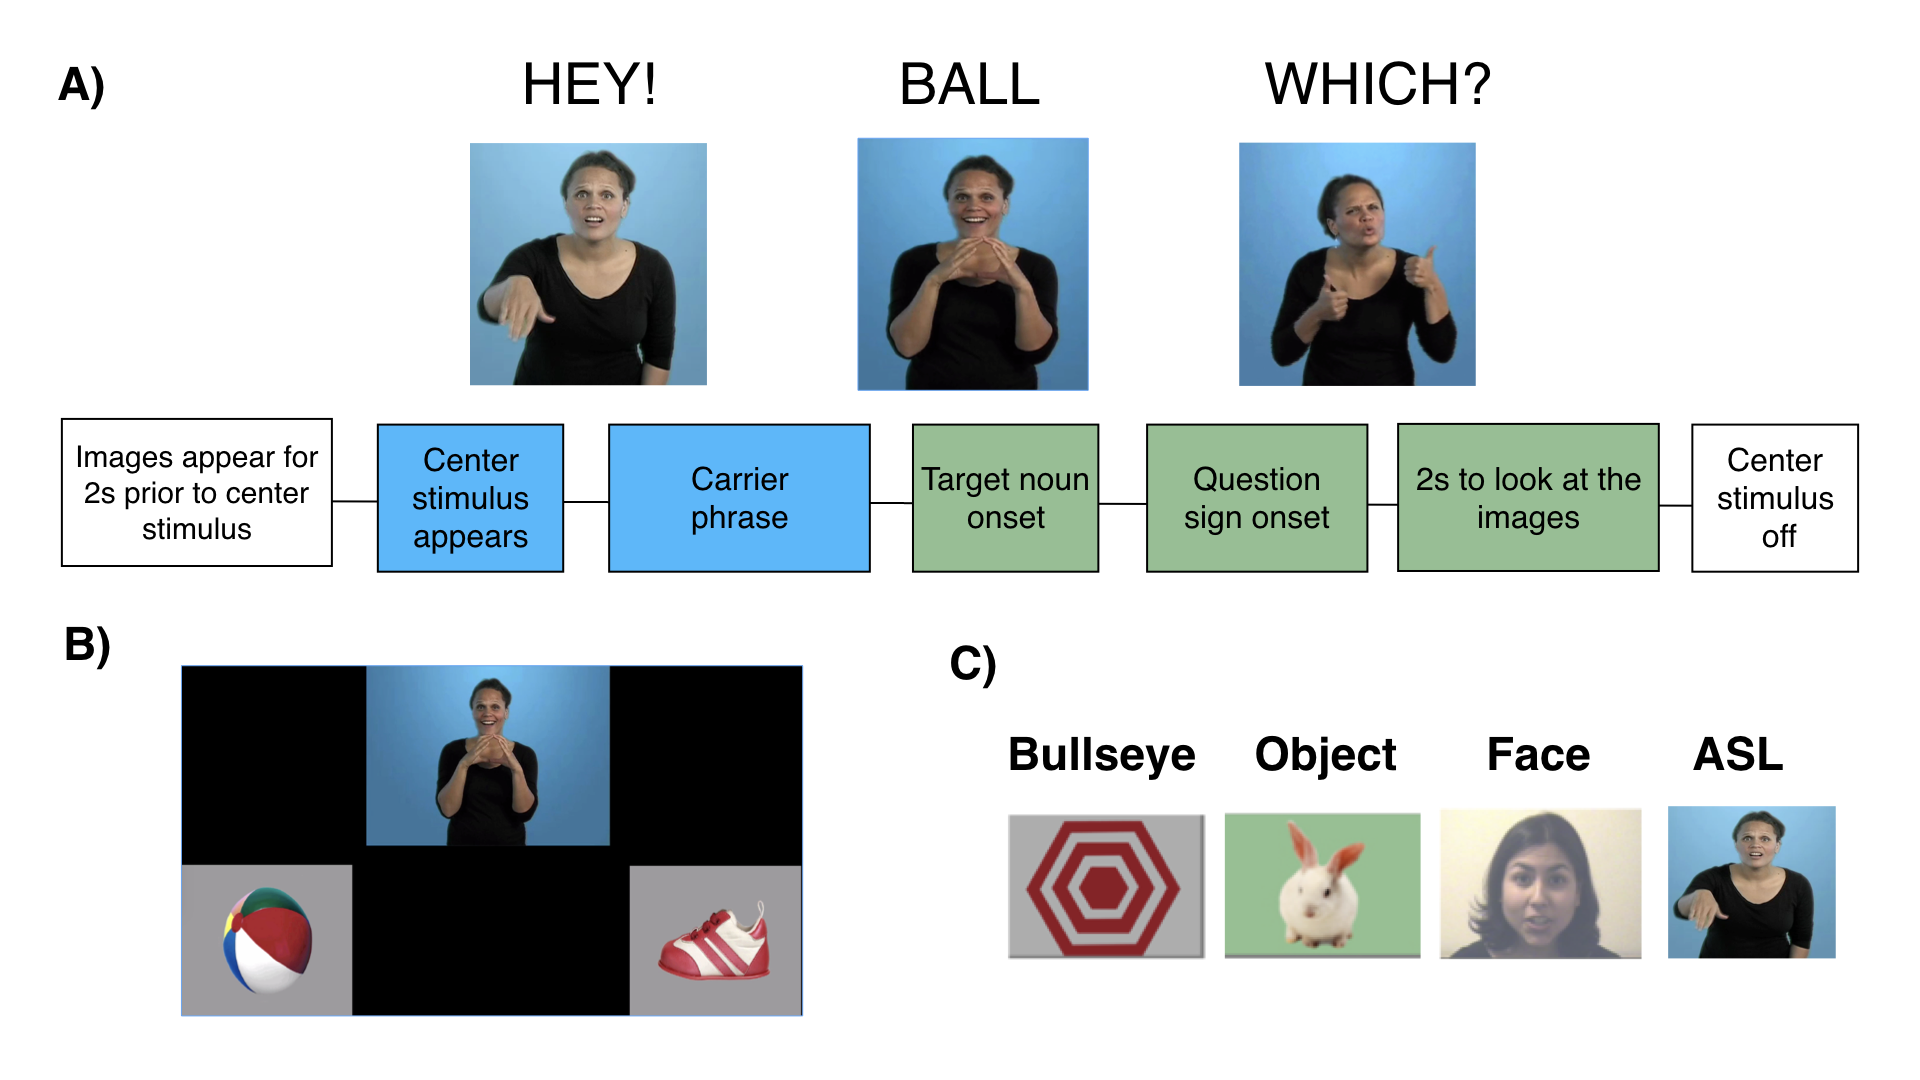
\includegraphics[width=0.9\linewidth]{/Users/kylemacdonald/Documents/Projects/speed-acc/writing/journal_submission/figures/figs_output//trio_stimuli} 

}

\caption{Stimuli for Experiments 1 and 2. Panel A shows the timecourse of the linguistic stimuli for a single trial for children learning American Sign Language. Panel B shows the layout of the fixation locations for all tasks: the center stimulus, the target, and the distracter. Panel C shows the four center stimulus items: a static geometric shape (Bullseye), a static image of a familiar object (Object), a person speaking (Face), a person signing (ASL).}\label{fig:trio-stim}
\end{figure}

There are differences between ASL and English question structures. All linguistic stimuli, however, shared the same trial structure: language to attract participants' attention followed by a sentence containing a target noun.

\emph{ASL linguistic stimuli.} We recorded two sets of ASL stimuli, using two valid ASL sentence structures for questions: 1) Sentence-initial wh-phrase: \enquote{HEY! WHICH {[}target noun{]}?} and 2) Sentence-final wh-phrase: \enquote{HEY! {[}target noun{]} WHICH?} Two female native ASL users recorded several tokens of each sentence in a child-directed register. Before each sentence, the signer produced a common attention-getting gesture. Mean sign length was 1254 ms, ranging from 693 ms to 1980 ms.

\emph{English linguistic stimuli.} All three tasks (Object, Bullseye, and Face) featured the same female speaker who used natural child-directed speech and said: \enquote{Look! Where's the (target word)?} The target words were: ball, banana, book, cookie, juice, and shoe. For the Face task, a female native English speaker was video-recorded as she looked straight ahead and said, \enquote{Look! Where's the (target word)?} Mean word length was 786.70 ms, ranging from 600 ms to 940 ms.

\emph{ASL and English visual stimuli.} The image set consisted of colorful digitized pictures of objects presented in fixed pairs with no phonological overlap (ASL task: cat---bird, car---book, bear---doll, ball---shoe; English tasks: book-shoe, juice-banana, cookie-ball). Side of target picture was counterbalanced across trials.

\hypertarget{design-and-procedure}{%
\subsubsection{Design and procedure}\label{design-and-procedure}}

\emph{Trial structure.} Children sat on their caregiver's lap and viewed the task on a screen while their gaze was recorded using a digital camcorder. On each trial, the child saw two images of familiar objects on the screen for two seconds before the center stimulus appeared. This time allowed the child to visually explore both images. Next, the target sentence -- which consisted of a carrier phrase, target noun, and question sign -- was presented, followed by two seconds without language to allow the child to respond to the signer's sentence. The trial structure of the Face, Object, and Bullseye tasks were highly similar: children were given two seconds to visually explore the objects prior to the appearance of the center stimulus, then processed a target sentence, and finally were given two seconds of silence to generate a response to the target noun. Participants saw 32 test trials with several filler trials interspersed to maintain interest.

\emph{Coding.} Participants' gaze patterns were videotaped and later coded frame-by-frame at 33-ms resolution by trained coders blind to target side. On each trial, coders indicated whether the eyes were fixated on the central signer, one of the images, shifting between pictures, or away (off), yielding a high-resolution record of eye movements aligned with target noun onset. Prior to coding, all trials were pre-screened to exclude those few trials on which the participant was inattentive or there was external interference. To assess inter-coder reliability, 25\% of the videos were re-coded. Agreement was scored at the level of individual frames of video and averaged 98\% on these reliability assessments.

\hypertarget{results}{%
\subsection{Results}\label{results}}

\begin{figure}[!t]

{\centering 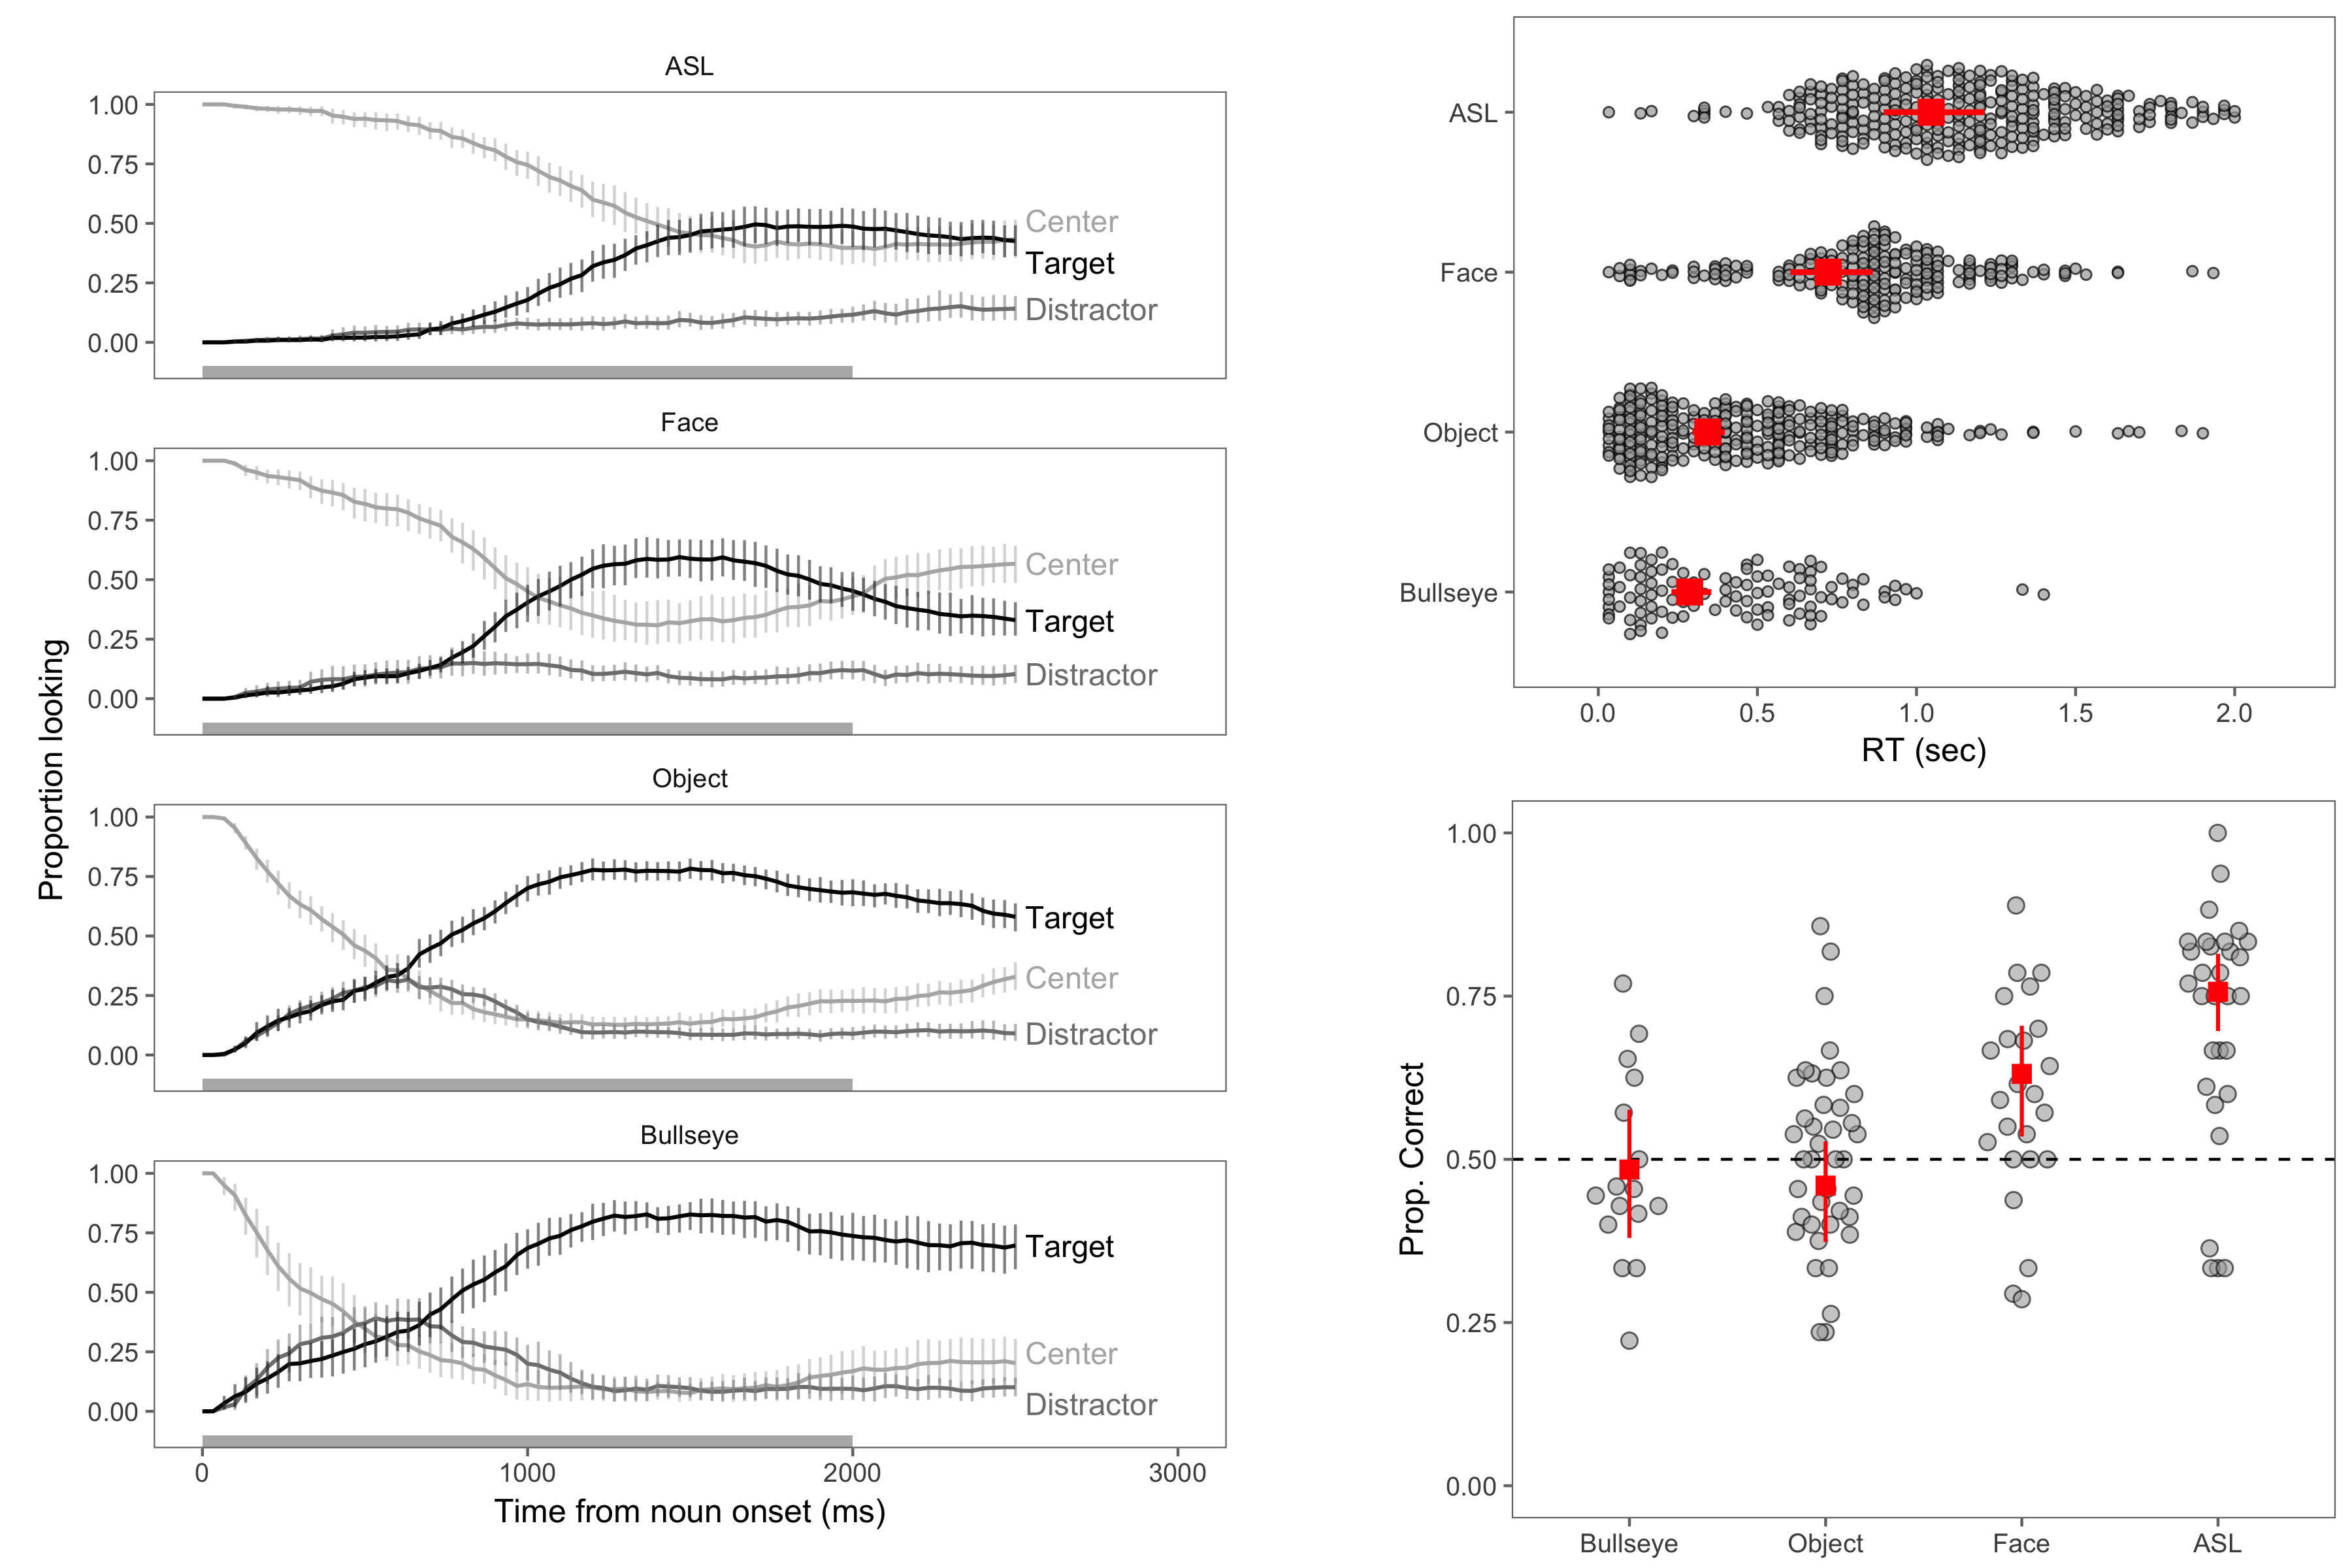
\includegraphics[width=0.9\linewidth]{/Users/kylemacdonald/Documents/Projects/speed-acc/writing/journal_submission/figures/figs_output//fig1_trio_behav} 

}

\caption{Timecourse looking, first shift Reaction Time (RT), and Accuracy results for children in Experiment 1. Panel A shows the overall looking to the center, target, and distracter stimulus for each context. Panel B shows the distribution of RTs for each participant. Each point represents a participant's average RT. The black squares represent the group means. And the error bars represent 95\% Highest Density Intervals around the group means. Panel C shows the same information but for the tendency of participants' first shifts to land on the language-consistent object.}\label{fig:speed-acc-trio-plot}
\end{figure}

\hypertarget{behavioral-analyses}{%
\subsubsection{Behavioral analyses}\label{behavioral-analyses}}

\emph{Timecourse looking.} The first question of interest was how do young ASL and English learners distribute attention across the three fixation locations while processing language in real-time? Figure~\ref{fig:speed-acc-trio-plot}A presents an overview of children's looking to each AOI for each processing context. This plot shows changes in the mean proportion of trials on which participants fixated the center stimulus, the target image, or the distracter image at every 33-ms interval of the stimulus sentence. At target-noun onset, children tended to look at the center stimulus. As the target noun unfolded, the mean proportion looking to the center decreased rapidly as participants shifted their gaze to the target or the distracter image. Proportion looking to the target increased sooner and reached a higher asymptote compared to proportion looking to the distracter for all four contexts.

After looking to the target image, participants tended to shift their gaze back to the center, shown by the increase in proportion looking to the center around two seconds after target-noun onset. There were several qualitative differences in looking behavior across the different center stimulus types. First, both ASL- and English-learners who processed sentences from a video of speaker spent more time looking to the center as indicated by the shallower slope on the curve for looks at the central stimulus. Second, when the center stimulus was a static geometric object (Bullseye) or a static familiar object (Object), spoken language learners were more likely to look at the distracter image, especially early in the timecourse of the target noun as indicated by the parallel increase in target and distracter-looking curves in Figure~\ref{fig:speed-acc-trio-plot}A. In contrast, spoken language learners in the Face context spent less time looking at the disracter, and ASL-learners rarely looked to the distracter image at any point in the trial. This pattern of behavior provides qualitative evidence that children adapated their gaze depending on language-relevant information available in the center stimulus loaction.

Based on a nonparametric cluster-based permutation analysis, the ASL learners' curve for looks at the central stimulus was significantly different from all other conditions (all \(p < .001\)). Within the spoken language groups, children's looking to a speaker's face was different from looking to the Bullseye and the Familar object (\(p < .001\)). Finally, the Object and Bullseye center-looking curves were not different from one another, with no significant differences at any point in the timecourse. Next, we ask how these different processing contexts changed the timing and accuracy of children's initial decisions to shift away from the center stimulus.

\emph{RT.} Figure~\ref{fig:speed-acc-trio-plot}B shows the full RT data distribution. To quantify differences across the groups, we fit a Bayesian linear mixed-effects regression predicting first shift RT as a function of center stimulus type controlling for age: \texttt{Log(RT) $\sim$ center stimulus type + age +  (1 | subject) + (1 | item)}. ASL learners generated slower RTs compared to all of the spoken English samples (\(\beta\) = 595.20 ms, 95\% HDI {[}444.60, 760.80{]}). Moreover, ASL learners' shifts were slower compared directly to children processing spoken language in the Face condition (\(\beta\) = 323.10 ms, 95\% HDI {[}132.30, 522.60{]}). Finally, children in the Face context shifted gaze slower compared to participants in the Object and Bullseye contexts (\(\beta\) = 408.20 ms, 95\% HDI {[}286.60, 546.20{]}).

\emph{Accuracy.} Next, we compared the accuracy of first shifts across the different tasks (Figure~\ref{fig:speed-acc-trio-plot}C) by fitting a mixed-effects logistic regression with the same specifications and contrasts as the RT model. We found that (a) ASL learners were more accurate compared to all of the spoken English samples (\(\beta\) = 0.23, 95\% HDI {[}0.17, 0.29{]}), (b) ASL learners were more accurate when directly compared to participants in the Face task (\(\beta\) = 0.13, 95\% HDI {[}0.04, 0.23{]}), (c) children learning spoken language were more accurate when processing language from dynamic video of a person speaking compared to the Object and Bullseye tasks (\(\beta\) = 0.16, 95\% HDI {[}0.07, 0.24{]}), and (d) English-learners' first shifts were no different from random responding in the Object (\(\beta\) = -0.04, 95\% HDI {[}-0.13, 0.03{]}) and Bullseye (\(\beta\) = -0.02, 95\% HDI {[}-0.12, 0.08{]}) contexts.

\hypertarget{model-based-analyses}{%
\subsubsection{Model-based analyses}\label{model-based-analyses}}

\begin{figure}[!t]

{\centering 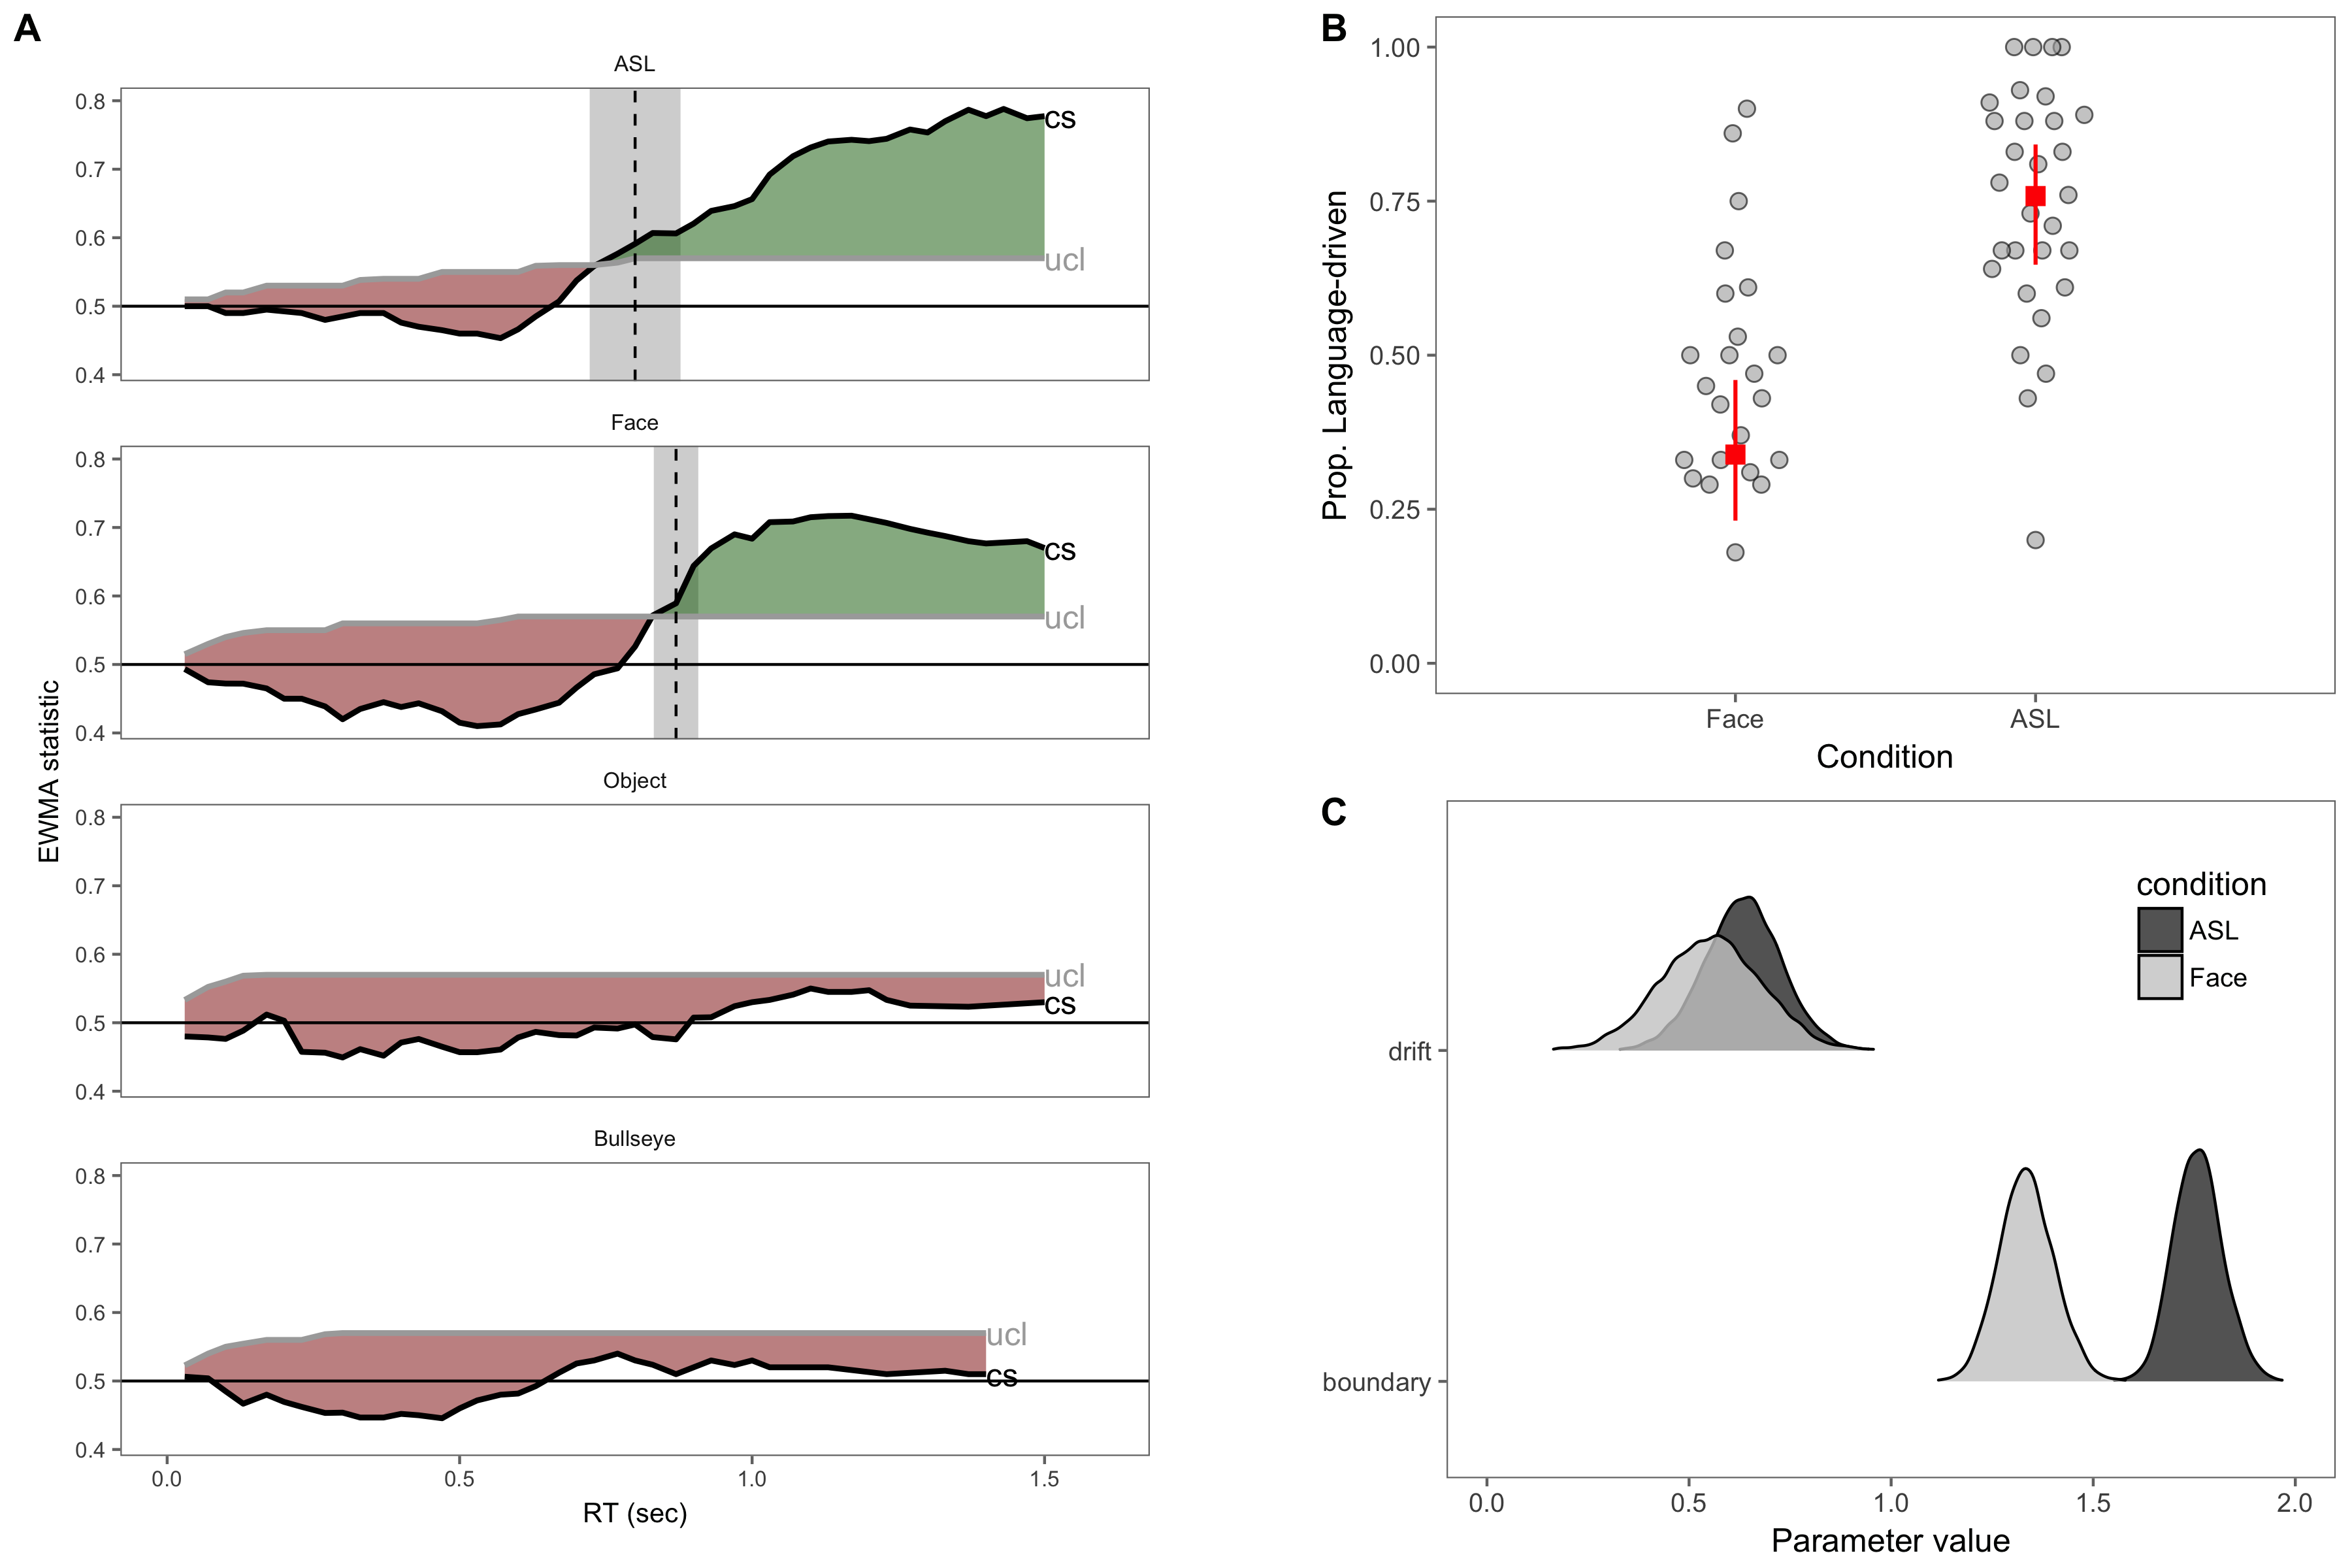
\includegraphics[width=0.9\linewidth]{/Users/kylemacdonald/Documents/Projects/speed-acc/writing/journal_submission/figures/figs_output//fig2_trio_models} 

}

\caption{Results for the model-based analyses in Experiment 1. Panel A shows a control chart representing the timecourse of the EWMA statistic. The black curve represents the evolution of the control statistic (CS) as a function of reaction time. The grey curve represents the upper control limit (UCL) or the pre-defined upper limit on random responding. The vertical dashed line is the median cutoff value (point in the RT distribution when children's gaze shifts were no longer random). The grey shaded area represents the 95\% Highest Density Interval around the estimate of the median cutoff point, and the shaded ribbons represent the classification of responses as guesses (red, below the UCL) and language-driven (green, above the UCL). Panel B shows a summary of the proportion of shifts that were categorized as language-driven for the Face and ASL processing contexts. Panel C shows the point estimate and 95\% Highest Density Intervals for the boundary and drift rate parameters for the Face and ASL contexts.}\label{fig:trio-model-plot}
\end{figure}

\emph{EWMA.} Our third question of interest was how the tendency to generate random vs.~language-driven gaze shifts evolved as a function of reaction time across the different processing contexts. Figure~\ref{fig:trio-model-plot}A shows changes in the control statistic (CS) and the upper control limit (UCL) as a function of RT. Each CS starts at chance performance and below the UCL. In the ASL and Face tasks, the CS value begins to increase with RTs around 0.7 seconds after noun onset and eventually crosses the UCL, indicating that responses \textgreater{} 0.7 sec were on average above chance levels. In contrast, the CS in the Object and Bullseye tasks never crossed the UCL, indicating that children's shifts were equally likely to land on the target or the distracter, regardless of when they were initiated. This result suggests that first shifts measured in the Bullseye/Object tasks were qualitatively different behaviors than those in the ASL and Face contexts. That is, these shifts are likely the result of a different generative process such as gathering more information about the referents in the visual world.

Next, we compared the EWMA model fits for participants in the ASL and Face processing contexts since these groups showed evidence of language-driven responding. We found that ASL learners generated fewer shifts when the CS was below the UCL compared to children learning spoken language (\(\beta\) = 0.14, 95\% HDI {[}0.08, 0.23{]}). This result indicates that ASL-learners were more likely to have gathered sufficient information about the linguistic signal prior to shifting gaze away from the language source. We found some evidence that ASL learners started producing language-driven shifts earlier in the RT distribution as indicated by the point at which the CS crossed the UCL (\(\beta\) = 0.22 sec, 95\% HDI {[}0.05, 0.39{]}), indicating that these children were less likely to generate early, random gaze shifts away from the signer.

\emph{HDDM.} We fit a hierarchical Drift Diffusion Model using only the gaze shifts categorized as language-driven by the EWMA. This allowed us to ask what underlying decision processes are likely to account for the measured differences in First Shift Accuracy and RT.\footnote{We chose not to interpret the HDDM fits for the Bullseye or Face tasks since there was no suggestion of any non-guessing signal from the EWMA analysis.} ASL learners had a higher estimate for the boundary separation parameter compared to children processing spoken English from a speaker (ASL boundary = 1.76, 95\% HDI {[}1.65, 1.88{]}; Face boundary = 1.34, 95\% HDI {[}1.21, 1.47{]}), with no overlap in the HDIs (see Figure~\ref{fig:trio-model-plot}C). This suggests that ASL learners' higher accuracy was driven by accumulating more evidence about the linguistic signal before generating an eye movement. We found high overlap for estimates of the drift rate parameter, indicating that both groups processed the linguistic information with similar efficiency (ASL drift = 0.63, 95\% HDI {[}0.44, 0.82{]}; Face drift = 0.55, 95\% HDI {[}0.30, 0.80{]}).

\hypertarget{discussion}{%
\subsection{Discussion}\label{discussion}}

There were several key findings from Study 1. First, focusing on only the spoken language learners, children were slower to shift gaze away from a speaker's face as compared to a static bullseye or a concrete familiar object. These gaze shifts, however, were more likely to land on the language-consistent object and more accurate overall, suggesting that fixating on the speaker supported language processing. Second, both behavioral and model-based analyses provided converging support that ASL learners were more sensitive to the value of delaying eye movements away from a language source. Compared to spoken language learners, ASL learners prioritized accuracy over speed (HDDM), produced more language-consistent shifts away from the center stimulus (EWMA and behavioral analyses). Importantly, we did not see evidence in the HDDM model fits that these accuracy differences could be explained by differential efficiency in processing the linguistic information. Instead, the pattern of results suggests that ASL learners increased their decision threshold to gather more information before shifting gaze away from the signer and to a named object.

We hypothesized that the Bullseye, Object, Face, and ASL contexts map onto a continuum of usefulness for language processing, ranging from least to most useful. In our data, we found that children tended to fixate longer on locations that were more language-relevant and in turn produced more accurate responses in these contexts. Moreover, we interpreted ASL learners' prioritization of accuracy above speed as an adaptive response. That is, to map referential language to the visual world in ASL involves competition for visual attention. When ASL learners choose to shift their gaze away from a signer, they are leaving an area that provides a great deal of useful information. Further, unlike children learning spoken languages, ASL learners cannot gather more of the linguistic signal if their gaze is directed away from a signer. Thus, it is reasonable that ASL learners would adapt the timing of their gaze shifts to gather additional information that increases certainty before seeking a named object.

These findings, however, were based on exploratory analyses, and our information-seeking explanation was developed post hoc to explain this pattern of results. There are several, potentially important differences between the stimuli, apparatus, and populations to point out. For example, the length of the target signs was on average longer and more variable than the English words. And while our prior work shows that children and adult signers tend to generate gaze shifts prior to sign offset (MacDonald et al., 2018), the differences between stimulus sets limit the strength of our interpretation and the generality of our account. Morever, we cannot make causal conclusions because of the observational nature of research comparing children who are learning different languages. Thus, we designed Experiment 2 to address these concerns by constructing a well-controlled situation that created information-seeking demands that are analogous on some dimensions to the modality-based differences in Experiment 1.

\hypertarget{experiment-2}{%
\section{Experiment 2}\label{experiment-2}}

In Experiment 2, we created an experimental context where we could manipulate the information-seeking demands in ways that parallel some aspects of the differences between young ASL- and English-learners.\footnote{See \url{https://osf.io/g8h9r/} for a pre-registration of the analysis plan.} We measured adults and children's eye movements during a real-time language comprehension task where participants processed sentences with familiar words (e.g., \enquote{Where's the ball?}) while looking at a simplified visual world with three fixation targets. Using a within-participants design, we manipulated the signal-to-noise ratio of the auditory signal by convolving the acoustic input with brown noise (random noise with higher energy at lower frequencies). We chose to manipulate background noise because it allowed us to increase the value of fixation on a speaker for the task of language comprehension, and it could be used with both children and adults. In Experiment 2, we chose to collect an adult sample so we could ask whether children might rely more on visual information because they have had less exposure to the target words and less experience processing language in the presence of background noise.

We predicted that processing speech in a noisy context would make listeners fixate longer on a speaker's face (slower reaction times), collect more visual information and generate a higher proportion of language-consistent responses (fewer responses classified as random by the EWMA model). We also predicted that children and adults would both adapt their gaze to gather additional visual information in the noisier auditory context, but that children might show an even stronger response in the noisy context since they have less-developed language and perceptual models as compared to adults.

\hypertarget{methods-1}{%
\subsection{Methods}\label{methods-1}}

\hypertarget{participants-1}{%
\subsubsection{Participants}\label{participants-1}}

Participants were native, monolingual English-learning children (\(n=\) 39; 22 F) and adults (\(n=\) 31; 22 F). All participants had no reported history of developmental or language delay and normal vision. 14 participants (11 children, 3 adults) were run but not included in the analysis because either the eye tracker failed to calibrate (2 children, 3 adults) or the participant did not complete the task (9 children). After excluding trials with less than 50\% valid data and RTs longer than two seconds, adults contributed on average 30.5 trials (min = 17, max = 32) to the analysis while children contributed on average 26.8 trials (min = 14, max = 32). There was no difference in the average number of trials contributed for the noisy (14.3) and clear auditory contexts (14.2). Based on time and resource constraints, we did not collect our planned sample size of 42 children in each age group (3-, 4-, and 5-year-olds); instead, we decided to use age as a continuous covariate and collected a single sample that included children across the entire age range.

\hypertarget{stimuli-1}{%
\subsubsection{Stimuli}\label{stimuli-1}}

\emph{Linguistic stimuli.} The video/audio stimuli were recorded in a sound-proof room and featured two female speakers who used natural child-directed speech and said one of two phrases: \enquote{Hey! Can you find the (target word)} or "Look! Where's the (target word). The target words were: ball, bunny, boat, bottle, cookie, juice, chicken, and shoe. The target words varied in length (shortest = 411.68 ms, longest = 779.62 ms) with an average length of 586.71 ms.

\emph{Noise manipulation}. To create the stimuli in the noise condition, we convolved each recording with Brown noise using the Audacity audio editor. The average signal-to-noise ratio (values greater than 0 dB indicate more signal than noise) in the noise condition was 2.87 dB compared to the clear condition, which was 35.05 dB.

\emph{Visual stimuli.} The image set consisted of colorful digitized pictures of objects presented in fixed pairs with no phonological overlap between the target and the distracter image (cookie-bottle, boat-juice, bunny-chicken, shoe-ball). The side of the target picture was counterbalanced across trials.

\hypertarget{design-and-procedure-1}{%
\subsubsection{Design and procedure}\label{design-and-procedure-1}}

Participants viewed the task on a screen while their gaze was tracked using an SMI RED corneal-reflection eye-tracker mounted on an LCD monitor, sampling at 30 Hz. The eye-tracker was first calibrated for each participant using a 6-point calibration. On each trial, participants saw two images of familiar objects on the screen for two seconds before the center stimulus appeared. Next, they processed the target sentence -- which consisted of a carrier phrase, a target noun, and a question -- followed by two seconds without language to allow for a response. Child participants saw 32 trials (16 noise trials; 16 clear trials) with several filler trials interspersed to maintain interest. Adult participants saw 64 trials (32 noise; 32 clear). The noise manipulation was presented in a blocked design with the order of block counterbalanced across participants.

\hypertarget{results-and-discussion}{%
\subsection{Results and Discussion}\label{results-and-discussion}}

\begin{figure}[!t]

{\centering 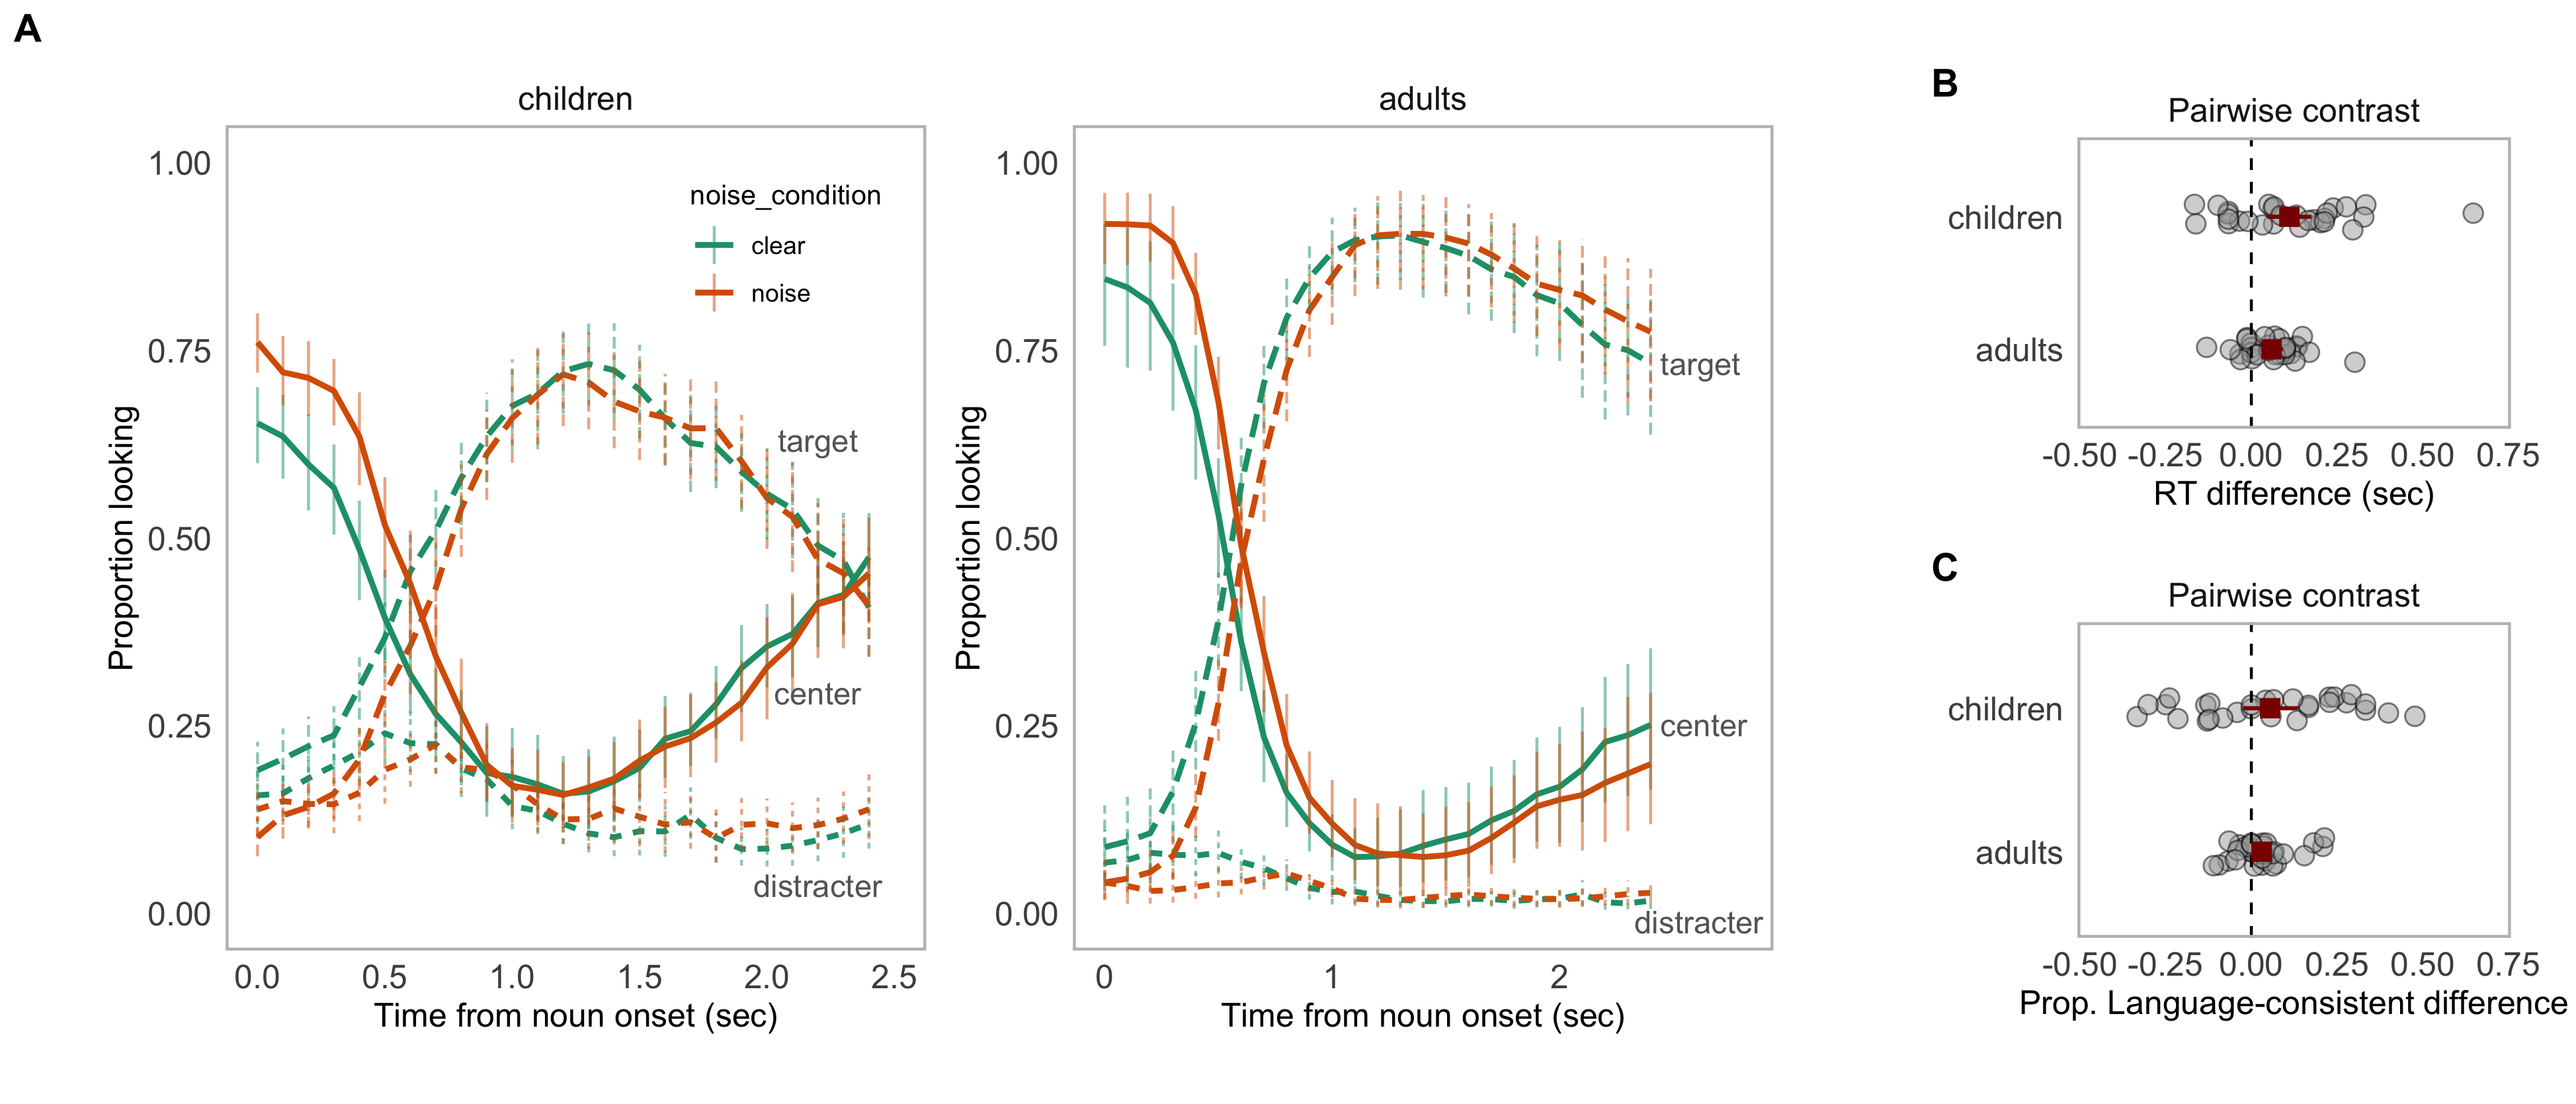
\includegraphics[width=0.9\linewidth]{/Users/kylemacdonald/Documents/Projects/speed-acc/writing/journal_submission/figures/figs_output//fig5_noise_behav} 

}

\caption{Behavioral results for children and adults in Experiment 2. Panel A shows the overall looking to the center, target, and distracter stimulus for each processing condition and age group. Panel B shows the distribution of pairwise contrasts between RTs in the noise and clear conditions. The square point represents the mean value for each mesure. The vertical dashed line represents the null model of zero condition difference. The width each point represents the 95\% HDI. Panel C shows the same information but for the tendency of participants' first shifts to land on the language-consistent object.}\label{fig:noise-acc-rt-plot}
\end{figure}

\hypertarget{behavioral-analyses-1}{%
\subsubsection{Behavioral analyses}\label{behavioral-analyses-1}}

\emph{Timecourse looking.} Figure~\ref{fig:noise-acc-rt-plot}A presents an overview of looking to the speaker, target, and distracter images for the noisy and clear processing contexts from the start of the target noun. Similar to the results in Experiment 1, participants tended to fixate on the speaker at target-noun onset. As the target noun unfolded, the mean proportion looking to the center decreased rapidly as participants shifted their gaze to the objects. Proportion looking to the target increased sooner and reached a higher asymptote compared to proportion looking to the distracter for both processing contexts and age groups. After looking to the target image, participants tended to shift their gaze back to the speaker as shown by the increase in center looking curve around 1 second.

There are several developmental differences to highlight. First, children tended to look more to the objects at noun onset, as indicated by the lower intercept of children's center-looking curves. Second, children's target looking curves reached a lower asymptote as compared to adults and they spent relatively more time fixating on the distracter image, whereas adults rarely looked at the unnamed object after 0.5 seconds in the timecourse of the trial. And third, children showed a stronger tendency to shift back to the speaker after looking to the named object.

Visual inspection of the center looking curves suggests a difference in looking behavior in the noisy processing context. Both children and adult's spent more time fixating on the speaker when the auditory signal was less reliable as indicated by the rightward shift of the center-looking curves in the noisy condition. A cluster-based permutation test confirmed that there was evidence of a significant difference in looking to the speaker between the Noisy and Clear conditions (\(p < .05\)). This pattern of behavior provides evidence that reducing the quality of the auditory signal increased looking to the speaker early in the timecourse of the target noun.

\emph{RT.} Figure~\ref{fig:noise-acc-rt-plot}B shows the full distribution of the estimated RT differences between each participants' performance in the noisy and clear contexts. Both children and adults were slower to identify the target in the noise condition (Children \(M_{noise}\) = 500.20 ms; Adult \(M_{noise}\) = 595.20 ms), as compared to the clear condition (Children \(M_{clear}\) = 455.70 ms Adult \(M_{clear}\) = 542.40 ms). RTs in the noise condition were 48.80 ms slower on average, with a 95\% HDI ranging from 3.70 ms to 96.30 ms, and not including the null value of zero condition difference. Older children responded faster than younger children (\(\beta_{age}\) = -0.44, {[}-0.74, -0.16{]}), with little evidence for an interaction between age and condition within the child sample.

\emph{Accuracy.} Next, we modeled adults and children's first shift accuracy using a mixed-effects logistic regression with the same specifications (Figure~\ref{fig:noise-acc-rt-plot}C). Both groups were more accurate than a model of random responding with the null value of \(0.5\) falling well outside the lower bound of the 95\% HDI for each group mean. Adults were more accurate (\(M_{adults} =\) 90\%) than children (\(M_{children} =\) 61\%). Interestingly, both groups showed evidence of higher accuracy in the noise condition: children (\(M_{noise}\) = 67\%; \(M_{clear}\) = 61\%) and adults (\(M_{noise}\) = 92\%; \(M_{clear}\) = 90\%). Accuracy in the noise condition was on average 4\% higher, with a 95\% HDI from -1\% to 12\%. Note that the null value of zero difference falls at the very edge of the HDI. But 95\% of the credible values are greater than zero, providing evidence for comparable, if not higher, accuracy in the noise condition. Within the child sample, there was no evidence of a main effect of age or an interaction between age and noise condition.

\hypertarget{model-based-analyses-1}{%
\subsubsection{Model-based analyses}\label{model-based-analyses-1}}

\begin{figure}[!t]

{\centering 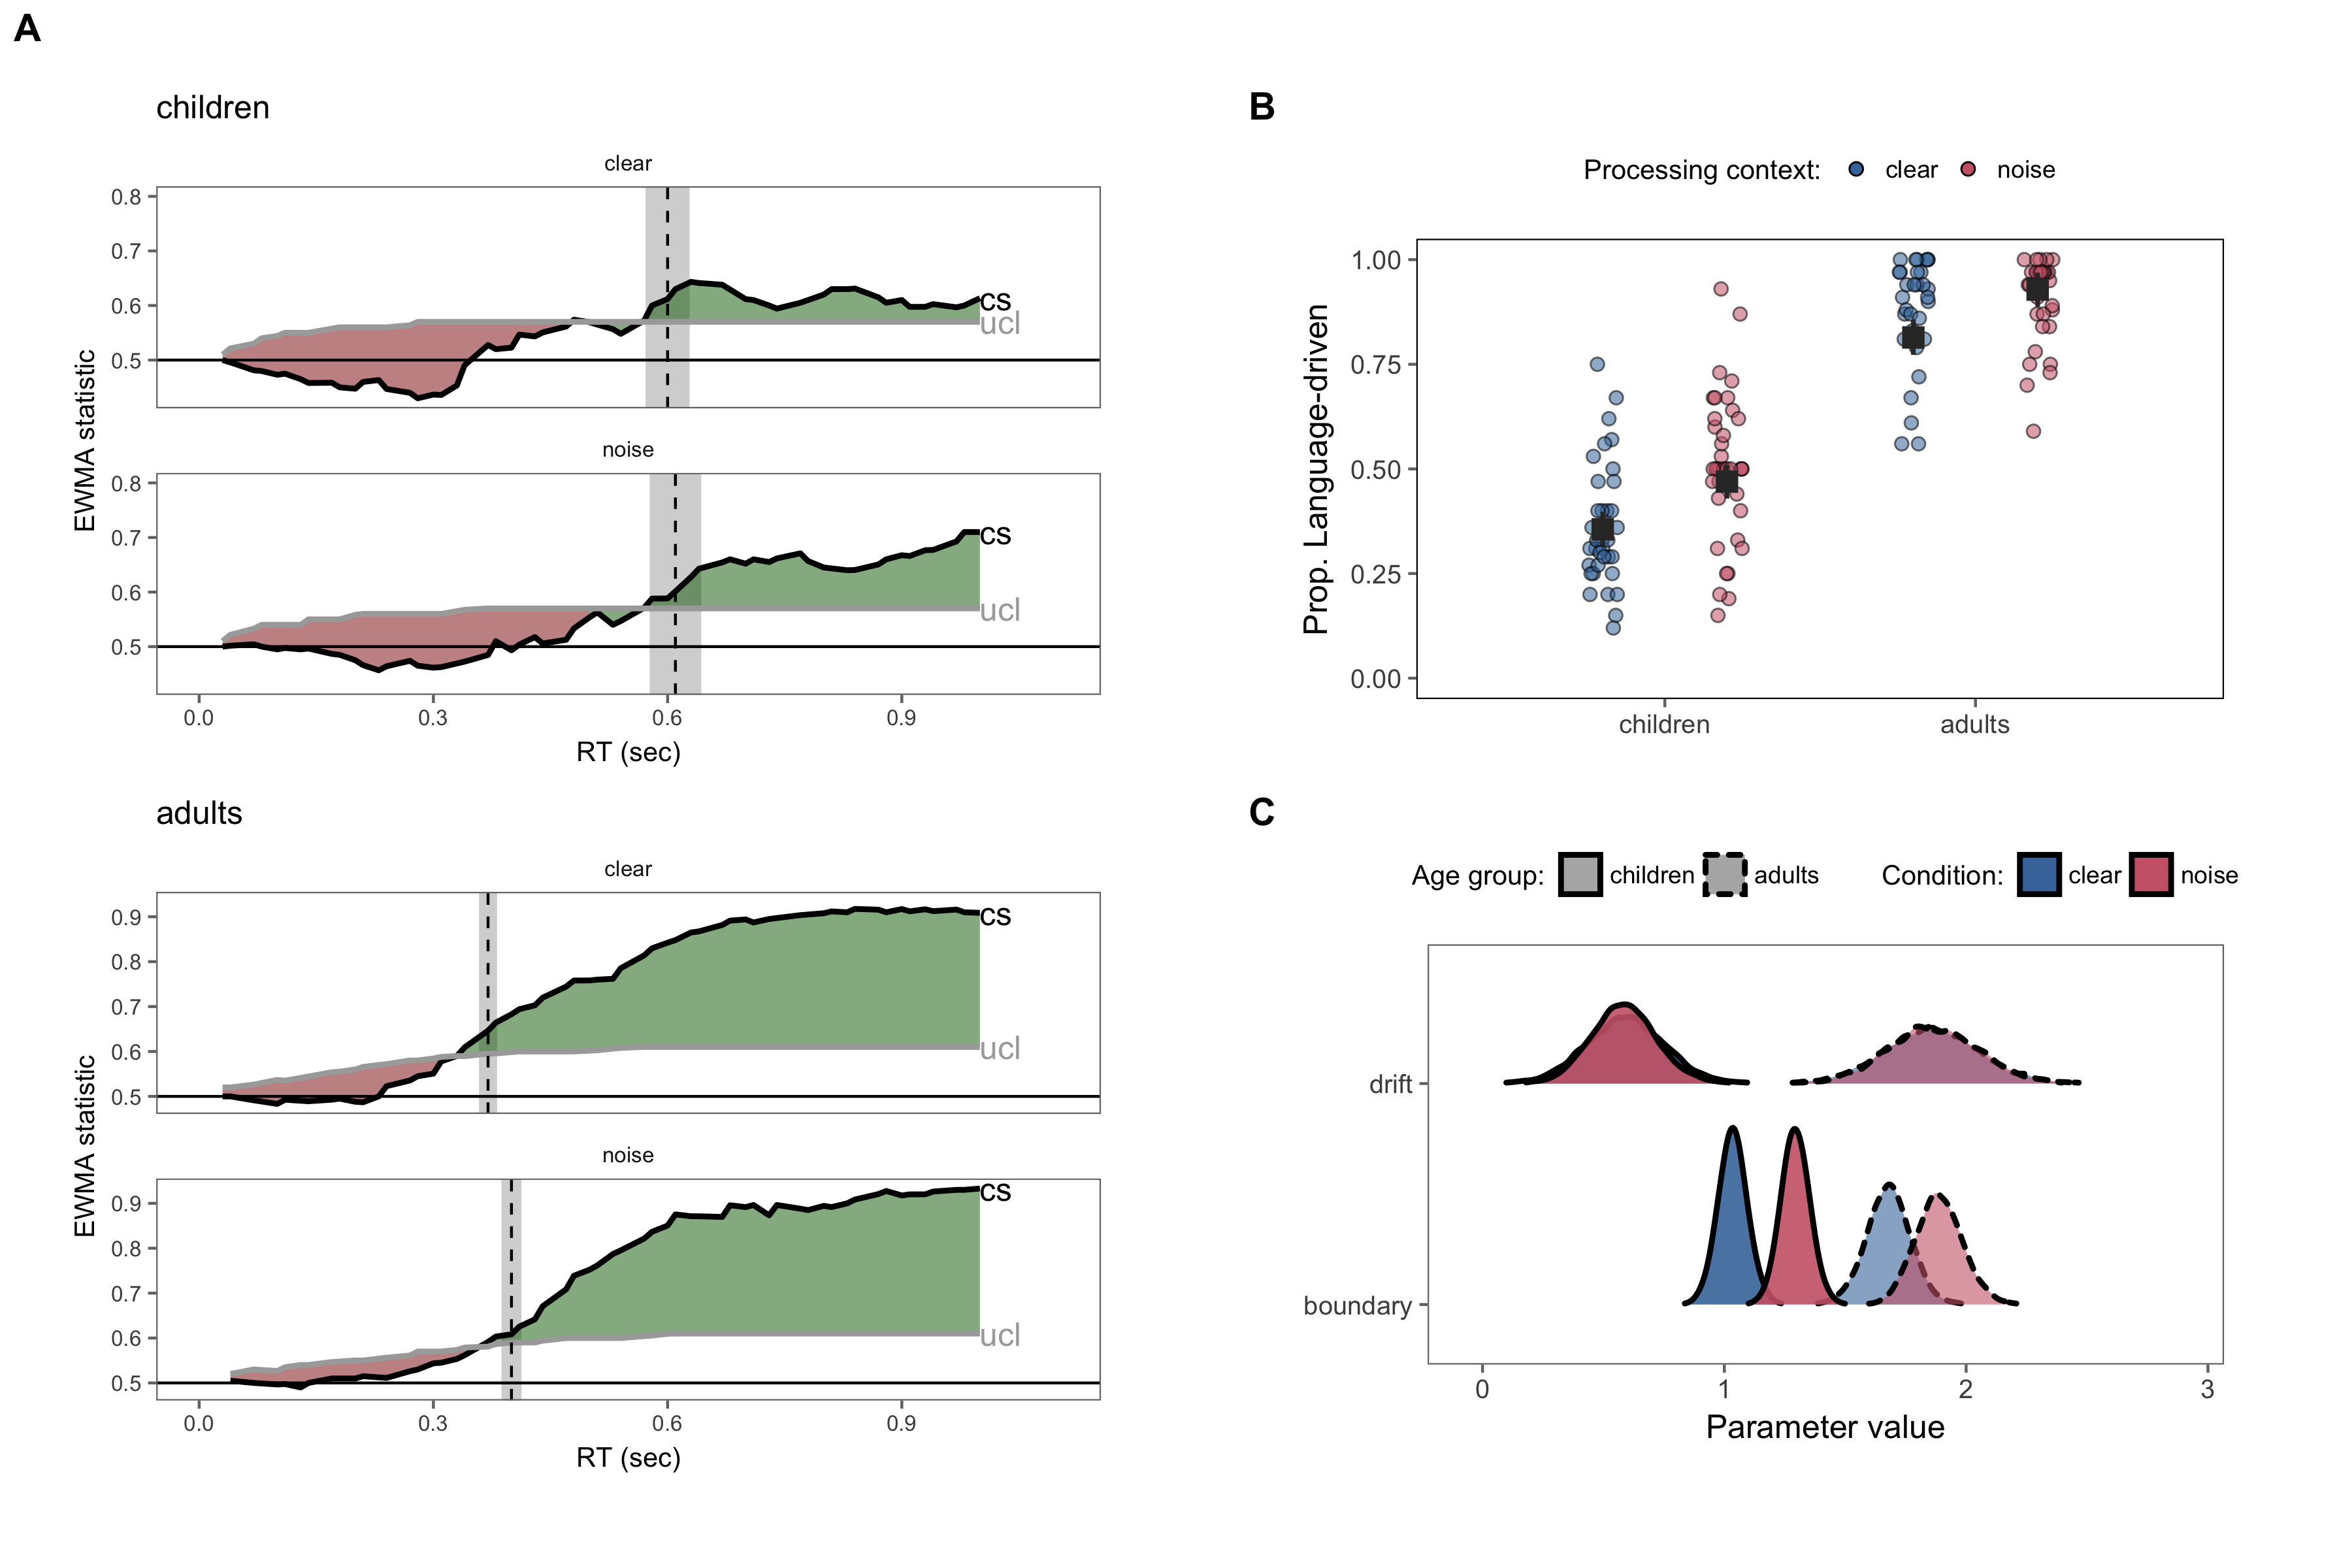
\includegraphics[width=0.9\linewidth]{/Users/kylemacdonald/Documents/Projects/speed-acc/writing/journal_submission/figures/figs_output//fig6_noise_models} 

}

\caption{Results for the model-based analyses for Experiment 2. The plotting conventions are the same as Figure 3.}\label{fig:noise-model-plots}
\end{figure}

\textbf{EWMA.} Figure~\ref{fig:noise-model-plots}A shows the proportion of shifts that the model classified as random vs.~language-driven for each age group and processing context. On average, 41\% (95\% HDI: 32\%, 50\%) of children's shifts were categorized as language-driven, which was significantly fewer than adults, 87\% (95\% HDI: 78\%, 96\%). Critically, processing speech in a noisy context caused both adults and children to generate a higher proportion of language-driven shifts (i.e., fewer random, exploratory shifts away from the speaker), with the 95\% HDI excluding the null value of zero condition difference (\(\beta_{noise}\) = 11\%, {[}7.00\%, 16\%{]}). Within the child sample, older children generated fewer random, early shifts (\(M_{age}\) = -0.21, {[}-0.35, -0.08{]}). There was no evidence of an interaction between age and condition. This pattern of results suggests that the noise condition caused participants to increase visual fixations to the language source, leading them to generate fewer exploratory, random shifts before they had accumulated sufficient information to respond in a language-consistent way.

\textbf{HDDM.} Figure~\ref{fig:noise-model-plots}B shows the full posterior distributions for the HDDM output. Children had lower estimates of drift rate (children \(M_{drift}\) = 0.59; adults \(M_{drift}\) = 1.90) and boundary separation (children \(M_{boundary}\) = 1.16; adults \(M_{boundary}\) = 1.67) as compared to adults, suggesting that children were less efficient and gathered less information. The noise manipulation selectively affected the boundary separation parameter, with higher estimates in the noise condition for both age groups (\(\beta_{noise}\) = 0.26, {[}0.10, 0.42{]}). This result suggests that participants in the noise condition prioritized information accumulation over speed when generating an eye movement in response to the incoming language, and this increased decision threshold led to higher accuracy. Moreover, the high overlap in estimates of drift rate suggests that participants were able to integrate the visual and auditory signals such that they could achieve a level of processing efficiency comparable to the clear processing context.

The behavioral and model-based results provide evidence for our information-seeking explanation of eye movements during grounded language comprehension. Processing speech in noise caused both children and adults to look longer at their social partner, which in turn, resulted in a higher proportion of language-consistent gaze shifts to a named object. Moreover, we observed a similar pattern of behavior in children and adults, with both groups producing more language-driven shifts (EWMA) and prioritized accuracy over speed (HDDM) in the more challenging noisy environment.

Our analysis plan was preregistered, but there were some cases where we deviated or did not predict a particular result. We successfully predicted that the noise manipulation would cause listeners to gather more information by looking longer at the speaker's face (slower RTs) and that this behavior would lead listeners to produce a higher proportion of language-driven shifts as indexed by the EWMA analysis. We did not, however, predict that first shifts would be \emph{more} language-consistent in the noisier context and that the noise manipulation would selectively affect the boundary separation parameter in the HDDM.

\hypertarget{general-discussion}{%
\section{General Discussion}\label{general-discussion}}

Language comprehension in grounded, social contexts provides children access to a rich set of multimodal cues that could support the linking of linguistic information to the world. But do children flexibly select what information to gather? In this work, we proposed that listeners adapt their gaze to seek visual information from their social partners when it was especially useful for language comprehension. We presented evidence for this explanation by measuring changes in how children chose to allocate visual attention across two diverse language processing contexts. In Experiment 1, we found that, compared to children learning spoken English, young ASL-learners delayed their gaze shifts away from a language source and produced a higher proportion of language-consistent eye movements. In Experiment 2, we showed that 3-5 year-olds and adults delayed the timing of gaze shifts away from a speaker's face while processing speech in a noisy auditory environment. This slower response resulted in fewer nonlanguage-driven eye movements and more language-consistent gaze shifts.

These results synthesize ideas from several research programs, including work on language-driven visual attention (Tanenhaus et al., 1995), goal-based accounts of vision during everyday tasks (Hayhoe \& Ballard, 2005; Henderson, 2017), and work on language perception as multisensory integration (Vigliocco et al., 2014). Our findings also parallel the results of several recent studies that measure the adaptation of visual processes in response to different auditory experiences. First, Heimler et al. (2015) compared deaf and hearing adults' performance on an oculomotor singleton detection paradigm where participants made speeded eye-movements to a unique target embedded among distracters that varied in saliency. Deaf adults were slower to generate a gaze shift away from the center fixation and, as a result, they were less affected by high saliency distracters. Second, McMurray, Farris-Trimble, and Rigler (2017) found that individuals with cochlear implants, who are consistently processing degraded auditory input, are more likely to delay the process of lexical access as measured by slower gaze shifts to named referents and fewer incorrect gaze shifts to phonological onset competitors. McMurray et al. (2017) also found that they could replicate these changes in adults with typical hearing by using noise-vocoded speech stimuli that shared features with the output of a cochlear implant.

Our findings also connect to the literature investigating how experience with a visual-manual language may change basic cognitive processes (see Bavelier, Dye, and Hauser (2006) for a review). The upshot of this work is that the effects of Deafness are dissociable from the effects of learning a signed language. Specifically, Deaf individuals show selective enhancement in peripheral visual attention as evidenced by higher sensitivity to peripheral distracters on spatial orienting tasks. In contrast, learning to sign results in several specific changes such as enhanced mental imagery (Emmorey, Kosslyn, \& Bellugi, 1993), mental rotation (Emmorey, Klima, \& Hickok, 1998), and face processing (Bettger, Emmorey, McCullough, \& Bellugi, 1997). The results of Experiment 1 suggest that ASL learners adapt the timing of when they disengage from a language source to increase their certainty before seeking named object. It is an open question as to whether ASL-learners' differential responding is best explained by a lack of access to auditory information or learning a visual-manual language.

Finally, our results dovetail with recent developmental work by Yurovsky et al. (2017). In their study, preschoolers, like adults, were able to integrate top-down expectations about the kinds of things speakers are likely to talk about with bottom-up cues from auditory perception. Yurovsky et al. (2017) situated this finding within the framework of modeling language as a \emph{noisy channel} where listeners combine expectations with perceptual data and weight each based on its reliability. In Experiment 2, we found a similar developmental parallel in language processing: that 3-5 year-olds, like adults, adapted their gaze patterns to seek additional visual information when the auditory signal became less reliable. This adaptation allowed listeners to generate comparable, if not more, language-consistent responses in the noisy context.

In additional to parallels, there were also clear patterns of developmental change between children and adults and within the child sample. First, adults were faster to respond to familiar words, generated more language-consistent shifts, and produced fewer early shifts before accumulating enough information to identify the target word. Older children also responded faster than younger children, replicating prior work showing that children's efficiency in processing familiar words increases over the first years of life (Fernald et al., 2006). Interestingly, older children did not generate more language-consistent shifts overall; instead they produced fewer early gaze shifts. This pattern of results suggests that what might be developing is children's ability to inhibit a behavior -- shifting gaze away from the language source -- that reduces access to information that helps identify the named referent. We did not design this study to test for the interaction between noise condition and children's age. Prior work, however, has found that older children become more robust to noise in the linguistic signal and show greater capacity to ignore irrelevant information in a sentence (Zangl \& Fernald, 2007). But it is still an open question as to how children's visual information seeking might change as they develop more efficient language processing skills that allow them to focus on the relevant information in the linguistic signal.

In sum, the work reported here shows that young listeners can seek visual information to support language comprehension. These results fit well with the interactive models of language perception reviewed in the Introduction (MacDonald \& Seidenberg, 2006; McClelland et al., 2006). These studies also highlight the value of integrating observational and experimental approaches. In Experiment 1, we compared language comprehension across populations of children who had very different language experiences (signed vs.~spoken) to generate a new explanation of observed differences in children's gaze dynamics. We were able to better understand this observational result by designing a well-controlled, follow-up experiment that allowed us to make stronger claims about the generality of our hypothesis.

\hypertarget{limitations-and-future-work}{%
\subsection{Limitations and future work}\label{limitations-and-future-work}}

Our results provide evidence that young listeners can adapt their gaze patterns to the demands of different processing environments to seek visual information from social partners that support language comprehension. We cannot, however, make claims about how children's behavior in our task (the Visual World Paradigm: VWP) would generalize to their decisions about how to distribute attention within real-world learning environments. There is a growing body of research showing meaningful links between children's gaze behavior in the VWP and relevant outcome measures such as vocabulary development (Fernald et al., 2006; Marchman \& Fernald, 2008; Rigler et al., 2015). Nonetheless, a valuable next step for our work would be to leverage tasks that move closer to the ecological context in which children process and learn language such as using head-mounted cameras and eye trackers that would allow measurement of where children choose to look during everyday interactions (Fausey, Jayaraman, \& Smith, 2016; Franchak, Kretch, Soska, \& Adolph, 2011).

This work has several other limitations. First, we chose to focus on a single decision about visual fixation to provide a window onto the dynamics of decision-making across different language processing contexts. But our analysis does not consider the rich information present in the gaze patterns that occur leading up to this decision. In our future work, we aim to measure how changes in the language environment might lead to shifts in the dynamics of gaze across a longer timescale. For example, perhaps listeners gather more information about the objects in the scene before the sentence in anticipation of allocating more attention to the speaker once they start to speak.

Second, we chose one instantiation of a noisy processing context -- random background noise. But we think our findings should generalize to settings where other kinds of noise -- e.g., uncertainty over a speaker's reliability or when processing accented speech -- make gathering visual information from the speaker more useful for language understanding. Moreover, we used a simple visual world, with only three places to look, and simple linguistic stimuli. Thus it remains an open question how these results might scale up to more complex language interactions and visual environments. It could be that looks to a speaker become even more useful for disambiguating reference in complex visual environments.

Third, we do not yet know what might be driving the population differences between children learning ASL and children learning spoken English found in Experiment 1. It could be that ASL-learners' massive experience dealing with competition for visual attention leads to changes in the deployment of eye movements during language comprehension. Or, it could be that the in-the-moment constraints of processing a visual language cause different fixation behaviors. This question could be addressed by studies that measure how quickly listeners adapt the dynamics of gaze when visual information becomes more useful. Another interesting approach would be to measure eye movements in hearing children learning both a signed and a spoken language (bimodal bilinguals). Our prior work found that hearing and Deaf native ASL learners show remarkably similar looking patterns over the time course of processing familiar signs (MacDonald et al., 2018). It would be interesting if hearing signers also prioritize language-consistent gaze shifts over speed of responding when comprehending their spoken language. This result would suggest that experience with a visual-manual language is changing a general response strategy, but if gaze dynamics looked different across language modalities within an individual, then this would favor an explanation based on the in-the-moment constraints of processing a visual-manual language in real-time.

Finally, our eye tracking paradigm removes an important component of successful communication: dynamic interaction between the speaker and listener. It is interesting to consider how speakers might adapt their behavior present the listener with useful visual information in challenging comprehension contexts. For example, in noisy environments, speakers will exaggerate mouth movements (Fitzpatrick, Kim, \& Davis, 2011) and increase the frequency of gestural cues such as head nodding (Munhall, Jones, Callan, Kuratate, \& Vatikiotis-Bateson, 2004), and parents exaggerate mouth movements during infant-directed speech (Green, Nip, Wilson, Mefferd, \& Yunusova, 2010). Moreover, observational studies of parent-child interactions in signed languages show variability in how sensitive adult signers are to the competing demands on children's visual attention (Harris \& Mohay, 1997). That is, some interactions contain many utterances that young signers miss because they are fixating on objects; whereas other interactions are marked by adaptations that accommodate the demands on visual attention by parents displacing signs onto the objects that are currently the focus of children's attention (similar to follow-in labeling effects Tomasello and Farrar, 1986). Thus it is an open question how interacting with a speaker that adapts to increase the availability and utility of visual information might change children's decisions about visual fixation.

\hypertarget{conclusion}{%
\subsection{Conclusion}\label{conclusion}}

In this paper, we presented an information-seeking explanation for the differences in the dynamics of eye movements during grounded signed vs.~spoken language comprehension. We started from an interesting, observational result: that ASL learners, compared to English-learning children, generate slower but more language-consistent gaze shifts away from a language source and to a named referent. We then tested the generality and causal claims of this explanation by experimentally manipulating the value of seeking visual information for language comprehension. The key finding is that young listeners can adapt the dynamics of their gaze to gather visual information when it is useful for language understanding.

\hypertarget{context-of-the-research}{%
\subsection{Context of the Research}\label{context-of-the-research}}

The current studies characterized children's eye movements as active decisions to gather language-relevant information, bringing together ideas from goal-based accounts of vision with work on multimodal language comprehension. We also think our approach could generalize in interesting ways to the language acquisition context. Consider that early in language learning, children acquire novel word-object links while also learning about visual object categories. Both of these tasks produce different goals that should, in turn, modulate children's decisions about where to allocate visual attention -- e.g., seeking nonlinguistic cues to reference such as eye gaze and pointing become critical when children are unfamiliar with the linguistic information. More generally, we think this approach presents a way forward for explaining decisions about visual fixation during language comprehension and acquisition across a broader range of processing contexts and at different stages of development.

\newpage

\hypertarget{references}{%
\section{References}\label{references}}

\setlength{\parindent}{-0.5in}
\setlength{\leftskip}{0.5in}

\hypertarget{refs}{}
\leavevmode\hypertarget{ref-allopenna1998tracking}{}%
Allopenna, P. D., Magnuson, J. S., \& Tanenhaus, M. K. (1998). Tracking the time course of spoken word recognition using eye movements: Evidence for continuous mapping models. \emph{Journal of Memory and Language}, \emph{38}(4), 419--439.

\leavevmode\hypertarget{ref-bavelier2006deaf}{}%
Bavelier, D., Dye, M. W., \& Hauser, P. C. (2006). Do deaf individuals see better? \emph{Trends in Cognitive Sciences}, \emph{10}(11), 512--518.

\leavevmode\hypertarget{ref-bettger1997enhanced}{}%
Bettger, J. G., Emmorey, K., McCullough, S. H., \& Bellugi, U. (1997). Enhanced facial discrimination: Effects of experience with american sign language. \emph{Journal of Deaf Studies and Deaf Education}, 223--233.

\leavevmode\hypertarget{ref-clark2009first}{}%
Clark, E. V. (2009). \emph{First language acquisition}. Cambridge University Press.

\leavevmode\hypertarget{ref-dahan2005looking}{}%
Dahan, D., \& Tanenhaus, M. K. (2005). Looking at the rope when looking for the snake: Conceptually mediated eye movements during spoken-word recognition. \emph{Psychonomic Bulletin \& Review}, \emph{12}(3), 453--459.

\leavevmode\hypertarget{ref-emmorey1998mental}{}%
Emmorey, K., Klima, E., \& Hickok, G. (1998). Mental rotation within linguistic and non-linguistic domains in users of american sign language. \emph{Cognition}, \emph{68}(3), 221--246.

\leavevmode\hypertarget{ref-emmorey1993visual}{}%
Emmorey, K., Kosslyn, S. M., \& Bellugi, U. (1993). Visual imagery and visual-spatial language: Enhanced imagery abilities in deaf and hearing asl signers. \emph{Cognition}, \emph{46}(2), 139--181.

\leavevmode\hypertarget{ref-erber1969interaction}{}%
Erber, N. P. (1969). Interaction of audition and vision in the recognition of oral speech stimuli. \emph{Journal of Speech and Hearing Research}, \emph{12}(2), 423--425.

\leavevmode\hypertarget{ref-estigarribia2007getting}{}%
Estigarribia, B., \& Clark, E. V. (2007). Getting and maintaining attention in talk to young children. \emph{Journal of Child Language}, \emph{34}(4), 799--814.

\leavevmode\hypertarget{ref-fausey2016faces}{}%
Fausey, C. M., Jayaraman, S., \& Smith, L. B. (2016). From faces to hands: Changing visual input in the first two years. \emph{Cognition}, \emph{152}, 101--107.

\leavevmode\hypertarget{ref-fernald2006picking}{}%
Fernald, A., Perfors, A., \& Marchman, V. A. (2006). Picking up speed in understanding: Speech processing efficiency and vocabulary growth across the 2nd year. \emph{Developmental Psychology}, \emph{42}(1), 98.

\leavevmode\hypertarget{ref-fernald2008looking}{}%
Fernald, A., Zangl, R., Portillo, A. L., \& Marchman, V. A. (2008). Looking while listening: Using eye movements to monitor spoken language. \emph{Developmental Psycholinguistics: On-Line Methods in Children's Language Processing}, \emph{44}, 97.

\leavevmode\hypertarget{ref-fitzpatrick2011effect}{}%
Fitzpatrick, M., Kim, J., \& Davis, C. (2011). The effect of seeing the interlocutor on auditory and visual speech production in noise. In \emph{Auditory-visual speech processing 2011}.

\leavevmode\hypertarget{ref-fourtassiword2018}{}%
Fourtassi, A., \& Frank, M. C. (2017). Word identification under multidomodal uncertainty. In \emph{Proceedings of the 39th annual conference of the cognitive science society}.

\leavevmode\hypertarget{ref-franchak2011head}{}%
Franchak, J. M., Kretch, K. S., Soska, K. C., \& Adolph, K. E. (2011). Head-mounted eye tracking: A new method to describe infant looking. \emph{Child Development}, \emph{82}(6), 1738--1750.

\leavevmode\hypertarget{ref-gabry2016rstanarm}{}%
Gabry, J., \& Goodrich, B. (2016). Rstanarm: Bayesian applied regression modeling via stan. R package version 2.10. 0.

\leavevmode\hypertarget{ref-gibson2013rational}{}%
Gibson, E., Bergen, L., \& Piantadosi, S. T. (2013). Rational integration of noisy evidence and prior semantic expectations in sentence interpretation. \emph{Proceedings of the National Academy of Sciences}, 201216438.

\leavevmode\hypertarget{ref-gold2000representation}{}%
Gold, J. I., \& Shadlen, M. N. (2000). Representation of a perceptual decision in developing oculomotor commands. \emph{Nature}, \emph{404}(6776), 390.

\leavevmode\hypertarget{ref-green2010lip}{}%
Green, J. R., Nip, I. S., Wilson, E. M., Mefferd, A. S., \& Yunusova, Y. (2010). Lip movement exaggerations during infant-directed speech. \emph{Journal of Speech, Language, and Hearing Research}, \emph{53}(6), 1529--1542.

\leavevmode\hypertarget{ref-harris1997learning}{}%
Harris, M., \& Mohay, H. (1997). Learning to look in the right place: A comparison of attentional behavior in deaf children with deaf and hearing mothers. \emph{The Journal of Deaf Studies and Deaf Education}, \emph{2}(2), 95--103.

\leavevmode\hypertarget{ref-hayhoe2005eye}{}%
Hayhoe, M., \& Ballard, D. (2005). Eye movements in natural behavior. \emph{Trends in Cognitive Sciences}, \emph{9}(4), 188--194.

\leavevmode\hypertarget{ref-heimler2015finding}{}%
Heimler, B., Zoest, W. van, Baruffaldi, F., Donk, M., Rinaldi, P., Caselli, M. C., \& Pavani, F. (2015). Finding the balance between capture and control: Oculomotor selection in early deaf adults. \emph{Brain and Cognition}, \emph{96}, 12--27.

\leavevmode\hypertarget{ref-henderson2017gaze}{}%
Henderson, J. M. (2017). Gaze control as prediction. \emph{Trends in Cognitive Sciences}, \emph{21}(1), 15--23.

\leavevmode\hypertarget{ref-henderson2007visual}{}%
Henderson, J. M., Brockmole, J. R., Castelhano, M. S., \& Mack, M. (2007). Visual saliency does not account for eye movements during visual search in real-world scenes. In \emph{Eye movements} (pp. 537--III). Elsevier.

\leavevmode\hypertarget{ref-hoppe2016learning}{}%
Hoppe, D., \& Rothkopf, C. A. (2016). Learning rational temporal eye movement strategies. \emph{Proceedings of the National Academy of Sciences}, \emph{113}(29), 8332--8337.

\leavevmode\hypertarget{ref-huettig2005word}{}%
Huettig, F., \& Altmann, G. T. (2005). Word meaning and the control of eye fixation: Semantic competitor effects and the visual world paradigm. \emph{Cognition}, \emph{96}(1), B23--B32.

\leavevmode\hypertarget{ref-kelly2010two}{}%
Kelly, S. D., Özyürek, A., \& Maris, E. (2010). Two sides of the same coin: Speech and gesture mutually interact to enhance comprehension. \emph{Psychological Science}, \emph{21}(2), 260--267.

\leavevmode\hypertarget{ref-liszkowski2012prelinguistic}{}%
Liszkowski, U., Brown, P., Callaghan, T., Takada, A., \& De Vos, C. (2012). A prelinguistic gestural universal of human communication. \emph{Cognitive Science}, \emph{36}(4), 698--713.

\leavevmode\hypertarget{ref-macdonald1978visual}{}%
MacDonald, J., \& McGurk, H. (1978). Visual influences on speech perception processes. \emph{Attention, Perception, \& Psychophysics}, \emph{24}(3), 253--257.

\leavevmode\hypertarget{ref-macdonald2018real}{}%
MacDonald, K., LaMarr, T., Corina, D., Marchman, V. A., \& Fernald, A. (2018). Real-time lexical comprehension in young children learning american sign language. \emph{Developmental Science}, e12672.

\leavevmode\hypertarget{ref-macdonald2006constraint}{}%
MacDonald, M. C., \& Seidenberg, M. S. (2006). Constraint satisfaction accounts of lexical and sentence comprehension. \emph{Handbook of Psycholinguistics}, \emph{2}, 581--611.

\leavevmode\hypertarget{ref-marchman2008speed}{}%
Marchman, V. A., \& Fernald, A. (2008). Speed of word recognition and vocabulary knowledge in infancy predict cognitive and language outcomes in later childhood. \emph{Developmental Science}, \emph{11}(3).

\leavevmode\hypertarget{ref-maris2007nonparametric}{}%
Maris, E., \& Oostenveld, R. (2007). Nonparametric statistical testing of eeg-and meg-data. \emph{Journal of Neuroscience Methods}, \emph{164}(1), 177--190.

\leavevmode\hypertarget{ref-mcclelland1986trace}{}%
McClelland, J. L., \& Elman, J. L. (1986). The trace model of speech perception. \emph{Cognitive Psychology}, \emph{18}(1), 1--86.

\leavevmode\hypertarget{ref-mcclelland2006there}{}%
McClelland, J. L., Mirman, D., \& Holt, L. L. (2006). Are there interactive processes in speech perception? \emph{Trends in Cognitive Sciences}, \emph{10}(8), 363--369.

\leavevmode\hypertarget{ref-mcmurray2017waiting}{}%
McMurray, B., Farris-Trimble, A., \& Rigler, H. (2017). Waiting for lexical access: Cochlear implants or severely degraded input lead listeners to process speech less incrementally. \emph{Cognition}, \emph{169}, 147--164.

\leavevmode\hypertarget{ref-munhall2004visual}{}%
Munhall, K. G., Jones, J. A., Callan, D. E., Kuratate, T., \& Vatikiotis-Bateson, E. (2004). Visual prosody and speech intelligibility: Head movement improves auditory speech perception. \emph{Psychological Science}, \emph{15}(2), 133--137.

\leavevmode\hypertarget{ref-nelson2005finding}{}%
Nelson, J. D. (2005). Finding useful questions: On bayesian diagnosticity, probability, impact, and information gain. \emph{Psychological Review}, \emph{112}(4), 979.

\leavevmode\hypertarget{ref-nelson2007probabilistic}{}%
Nelson, J. D., \& Cottrell, G. W. (2007). A probabilistic model of eye movements in concept formation. \emph{Neurocomputing}, \emph{70}(13-15), 2256--2272.

\leavevmode\hypertarget{ref-peelle2015prediction}{}%
Peelle, J. E., \& Sommers, M. S. (2015). Prediction and constraint in audiovisual speech perception. \emph{Cortex}, \emph{68}, 169--181.

\leavevmode\hypertarget{ref-ratcliff2015individual}{}%
Ratcliff, R., \& Childers, R. (2015). Individual differences and fitting methods for the two-choice diffusion model of decision making. \emph{Decision}, \emph{2}(4), 237--279.

\leavevmode\hypertarget{ref-rigler2015slow}{}%
Rigler, H., Farris-Trimble, A., Greiner, L., Walker, J., Tomblin, J. B., \& McMurray, B. (2015). The slow developmental time course of real-time spoken word recognition. \emph{Developmental Psychology}, \emph{51}(12), 1690.

\leavevmode\hypertarget{ref-salverda2011goal}{}%
Salverda, A. P., Brown, M., \& Tanenhaus, M. K. (2011). A goal-based perspective on eye movements in visual world studies. \emph{Acta Psychologica}, \emph{137}(2), 172--180.

\leavevmode\hypertarget{ref-shinoda2001controls}{}%
Shinoda, H., Hayhoe, M. M., \& Shrivastava, A. (2001). What controls attention in natural environments? \emph{Vision Research}, \emph{41}(25-26), 3535--3545.

\leavevmode\hypertarget{ref-tanenhaus1995integration}{}%
Tanenhaus, M. K., Spivey-Knowlton, M. J., Eberhard, K. M., \& Sedivy, J. C. (1995). Integration of visual and linguistic information in spoken language comprehension. \emph{Science}, \emph{268}(5217), 1632.

\leavevmode\hypertarget{ref-tomasello1986joint}{}%
Tomasello, M., \& Farrar, M. J. (1986). Joint attention and early language. \emph{Child Development}, 1454--1463.

\leavevmode\hypertarget{ref-torralba2006contextual}{}%
Torralba, A., Oliva, A., Castelhano, M. S., \& Henderson, J. M. (2006). Contextual guidance of eye movements and attention in real-world scenes: The role of global features in object search. \emph{Psychological Review}, \emph{113}(4), 766.

\leavevmode\hypertarget{ref-triesch2003you}{}%
Triesch, J., Ballard, D. H., Hayhoe, M. M., \& Sullivan, B. T. (2003). What you see is what you need. \emph{Journal of Vision}, \emph{3}(1), 9--9.

\leavevmode\hypertarget{ref-vandekerckhove2007fitting}{}%
Vandekerckhove, J., \& Tuerlinckx, F. (2007). Fitting the ratcliff diffusion model to experimental data. \emph{Psychonomic Bulletin \& Review}, \emph{14}(6), 1011--1026.

\leavevmode\hypertarget{ref-venker2013individual}{}%
Venker, C. E., Eernisse, E. R., Saffran, J. R., \& Weismer, S. E. (2013). Individual differences in the real-time comprehension of children with asd. \emph{Autism Research}, \emph{6}(5), 417--432.

\leavevmode\hypertarget{ref-vigliocco2014language}{}%
Vigliocco, G., Perniss, P., \& Vinson, D. (2014). Language as a multimodal phenomenon: Implications for language learning, processing and evolution. The Royal Society.

\leavevmode\hypertarget{ref-wiecki2013hddm}{}%
Wiecki, T. V., Sofer, I., \& Frank, M. J. (2013). HDDM: Hierarchical bayesian estimation of the drift-diffusion model in python. \emph{Frontiers in Neuroinformatics}, \emph{7}, 14.

\leavevmode\hypertarget{ref-yee2006eye}{}%
Yee, E., \& Sedivy, J. C. (2006). Eye movements to pictures reveal transient semantic activation during spoken word recognition. \emph{Journal of Experimental Psychology: Learning, Memory, and Cognition}, \emph{32}(1), 1.

\leavevmode\hypertarget{ref-yurovsky2017preschoolers}{}%
Yurovsky, D., Case, S., \& Frank, M. C. (2017). Preschoolers flexibly adapt to linguistic input in a noisy channel. \emph{Psychological Science}, \emph{28}(1), 132--140.

\leavevmode\hypertarget{ref-zangl2007increasing}{}%
Zangl, R., \& Fernald, A. (2007). Increasing flexibility in children's online processing of grammatical and nonce determiners in fluent speech. \emph{Language Learning and Development}, \emph{3}(3), 199--231.

\clearpage
\makeatletter
\efloat@restorefloats
\makeatother


\begin{appendix}
\hypertarget{experiment-1}{%
\section{Experiment 1}\label{experiment-1}}

\begin{table}[h]
\begin{center}
\begin{threeparttable}
\caption{\label{tab:trio-rt-model}Output of the regression predicting reaction time (milliseconds) as a function of center stimulus type in Experiment 1.}
\begin{tabular}{lll}
\toprule
Center Stimulus Type & \multicolumn{1}{c}{Mean RT} & \multicolumn{1}{c}{95\% HDI}\\
\midrule
Bullseye & 288.71 & [229.8, 355.17]\\
Object & 344.51 & [295.71, 397.31]\\
Face & 724.78 & [603.2, 862.81]\\
ASL & 1,047.89 & [897.29, 1213.52]\\
\bottomrule
\end{tabular}
\end{threeparttable}
\end{center}
\end{table}

\begin{table}[h]
\begin{center}
\begin{threeparttable}
\caption{\label{tab:trio-acc-model}Output of the logistic regression predicting accuracy as a function of center stimulus type in Experiment 1.}
\begin{tabular}{lll}
\toprule
Center Stimulus Type & \multicolumn{1}{c}{Mean Accuracy} & \multicolumn{1}{c}{95\% HDI}\\
\midrule
Object & 0.46 & [0.37, 0.53]\\
Bullseye & 0.48 & [0.38, 0.58]\\
Face & 0.63 & [0.54, 0.7]\\
ASL & 0.76 & [0.7, 0.81]\\
\bottomrule
\end{tabular}
\end{threeparttable}
\end{center}
\end{table}

\begin{table}[h]
\begin{center}
\begin{threeparttable}
\caption{\label{tab:trio-acc-contrasts}Output of the model estimating differences in Accuracy for specific contrasts of interest in Experiment 1.}
\begin{tabular}{lll}
\toprule
Contrast & \multicolumn{1}{c}{Mean Difference Accuracy} & \multicolumn{1}{c}{95\% HDI}\\
\midrule
Object vs. Chance & -0.04 & [-0.13, 0.03]\\
Bullseye vs. Chance & -0.02 & [-0.12, 0.08]\\
ASL vs. Face & 0.13 & [0.04, 0.23]\\
Face vs. Object/Bullseye & 0.16 & [0.07, 0.24]\\
ASL vs. English & 0.23 & [0.17, 0.29]\\
\bottomrule
\end{tabular}
\end{threeparttable}
\end{center}
\end{table}

\begin{table}[h]
\begin{center}
\begin{threeparttable}
\caption{\label{tab:trio-rt-contrasts}Output of the model estimating differences in RT for specific contrasts of interest in Experiment 1.}
\begin{tabular}{lll}
\toprule
Contrast & \multicolumn{1}{c}{Mean Difference RT} & \multicolumn{1}{c}{95\% HDI}\\
\midrule
ASL vs. Face & 323.10 & [132.3, 522.6]\\
Face vs. Object/Bullseye & 408.20 & [286.6, 546.2]\\
ASL vs. English & 595.20 & [444.6, 760.8]\\
\bottomrule
\end{tabular}
\end{threeparttable}
\end{center}
\end{table}

\begin{table}[h]
\begin{center}
\begin{threeparttable}
\caption{\label{tab:trio-ewma-cuts}Output of the model estimating the point in the Reaction Time distribution when children's Exponentially Weighted Moving Average statistic crossed the pre-defined guessing threshold for the ASL and Face center stimulus types in Experiment 1.}
\begin{tabular}{lll}
\toprule
Center Stimulus Type & \multicolumn{1}{c}{Mean EWMA Cut Point} & \multicolumn{1}{c}{95\% HDI}\\
\midrule
ASL & 0.68 & [0.59, 0.78]\\
Face & 0.90 & [0.77, 1.03]\\
\bottomrule
\end{tabular}
\end{threeparttable}
\end{center}
\end{table}

\begin{table}[h]
\begin{center}
\begin{threeparttable}
\caption{\label{tab:trio-guess-cuts}Output of the model estimating the mean proportion of shifts categorized as language-driven by the Exponentially Weighted Moving Average model for the ASL and Face center stimulus types in Experiment 1.}
\begin{tabular}{lll}
\toprule
Center Stimulus Type & \multicolumn{1}{c}{Mean Language-driven} & \multicolumn{1}{c}{95\% HDI}\\
\midrule
Face & 0.34 & [0.23, 0.46]\\
Asl & 0.75 & [0.65, 0.84]\\
\bottomrule
\end{tabular}
\end{threeparttable}
\end{center}
\end{table}

\begin{table}[h]
\begin{center}
\begin{threeparttable}
\caption{\label{tab:trio-hddm}Summary of the Drift Diffusion Model output for the drift rate and boundary separation parameters for both all four center stimulus types in Experiment 1.}
\begin{tabular}{llll}
\toprule
Parameter & \multicolumn{1}{c}{Center Stim Type} & \multicolumn{1}{c}{Mean Param Estimate} & \multicolumn{1}{c}{95\% HDI}\\
\midrule
Boundary & Face & 1.34 & [1.21, 1.47]\\
Boundary & ASL & 1.76 & [1.65, 1.88]\\
Drift & Face & 0.55 & [0.3, 0.8]\\
Drift & ASL & 0.63 & [0.44, 0.82]\\
\bottomrule
\end{tabular}
\end{threeparttable}
\end{center}
\end{table}

\hypertarget{experiment-2}{%
\section{Experiment 2}\label{experiment-2}}

\begin{table}[h]
\begin{center}
\begin{threeparttable}
\caption{\label{tab:noise-acc-model}Output of the logistic regression predicting accuracy as a function of noise condition and age group in Experiment 2.}
\begin{tabular}{llll}
\toprule
Noise Condition & \multicolumn{1}{c}{Age Group} & \multicolumn{1}{c}{Mean Accuracy} & \multicolumn{1}{c}{95\% HDI}\\
\midrule
Clear & children & 0.61 & [0.54, 0.68]\\
Noise & children & 0.67 & [0.6, 0.74]\\
Clear & adults & 0.90 & [0.87, 0.93]\\
Noise & adults & 0.92 & [0.89, 0.95]\\
\bottomrule
\end{tabular}
\end{threeparttable}
\end{center}
\end{table}

\begin{table}[h]
\begin{center}
\begin{threeparttable}
\caption{\label{tab:noise-rt-model}Output of the regression estimating reaction times (milliseconds) as a function of noise condition and age group in Experiment 2.}
\begin{tabular}{llll}
\toprule
Noise Condition & \multicolumn{1}{c}{Age Group} & \multicolumn{1}{c}{Mean RT} & \multicolumn{1}{c}{95\% HDI}\\
\midrule
Clear & children & 455.70 & [407, 503.6]\\
Noise & children & 500.20 & [446.6, 555.6]\\
Clear & adults & 542.40 & [486.2, 602.4]\\
Noise & adults & 595.20 & [532.4, 665.3]\\
\bottomrule
\end{tabular}
\end{threeparttable}
\end{center}
\end{table}

\begin{table}[h]
\begin{center}
\begin{threeparttable}
\caption{\label{tab:noise-guess-cuts}Output of the model estimating the mean proportion of shifts categorized as language-driven by the Exponentially Weighted Moving Average model for the each noise condition and age group in Experiment 2.}
\begin{tabular}{llll}
\toprule
Noise Condition & \multicolumn{1}{c}{Age Group} & \multicolumn{1}{c}{Mean Language-driven} & \multicolumn{1}{c}{95\% HDI}\\
\midrule
Clear & children & 0.36 & [0.32, 0.4]\\
Noise & children & 0.47 & [0.43, 0.51]\\
Clear & adults & 0.81 & [0.77, 0.86]\\
Noise & adults & 0.93 & [0.89, 0.97]\\
\bottomrule
\end{tabular}
\end{threeparttable}
\end{center}
\end{table}

\begin{table}[h]
\begin{center}
\begin{threeparttable}
\caption{\label{tab:noise-hddm}Summary of the Drift Diffusion Model output for the drift rate and boundary separation parameters for both processing contexts and age groups in Experiment 2.}
\begin{tabular}{llll}
\toprule
Parameter & \multicolumn{1}{c}{Age Group} & \multicolumn{1}{c}{Mean Parameter Estimate} & \multicolumn{1}{c}{95\% HDI}\\
\midrule
Boundary & Children & 1.16 & [0.94, 1.39]\\
Boundary & Adults & 1.67 & [1.49, 1.84]\\
Drift & Children & 0.59 & [0.3, 0.89]\\
Drift & Adults & 1.90 & [1.51, 2.3]\\
\bottomrule
\end{tabular}
\end{threeparttable}
\end{center}
\end{table}
\end{appendix}


\end{document}
